%**************************************************************
\section{Casi d'uso}
\label{sec:casi-uso}

I casi d'uso studiati per il prodotto sono stati realizzati sotto forma testuale, per una spiegazione dettagliata, e sotto forma di diagrammi.
Ciascuno testo descrittivo di un caso d'uso ne indica:
\begin{itemize}
    \item il \emph{codice identificativo}, nella forma $UCx.y.z$ con $x$, $y$ e $z$ numeri naturali;
    \item il \emph{nome}, che introduce brevemente il contesto applicativo del caso d'uso;
    \item gli \emph{attori principali} e \emph{attori secondari} (quest'ultimi se presenti), rispettivamente coloro che compiono l'azione indicata nel caso d'uso e coloro che invece aiutano a raggiungere le post-condizioni;
    \item lo \emph{scenario principale}, ovvero cosa può compiere l'utente con questo caso d'uso;
    \item le \emph{precondizioni}, ovvero lo stato del sistema antecedente l'esecuzione della funzionalità descritta;
    \item le \emph{postcondizioni}, ovvero lo stato del sistema alla fine dell'esecuzione della funzionalità descritta;
    \item le \emph{estensioni} (se presenti), ovvero una lista di casi d'uso che possono verificarsi sotto determinate condizioni che non permettono di raggiungere le postcondizioni indicate dal caso d'uso d'origine;
    \item le \emph{generalizzazioni} (se presenti), ovvero una lista di casi d'uso di cui il caso d'uso è implementazione più dettagliata.
\end{itemize}
I diagrammi dei casi d'uso (in inglese \emph{Use Case Diagram}) sono diagrammi realizzati in \gls{uml} dedicati alla descrizione delle funzioni o servizi offerti da un sistema, così come sono percepiti e utilizzati dagli attori che interagiscono col sistema stesso.

\begin{figure}[!h] 
    \centering 
    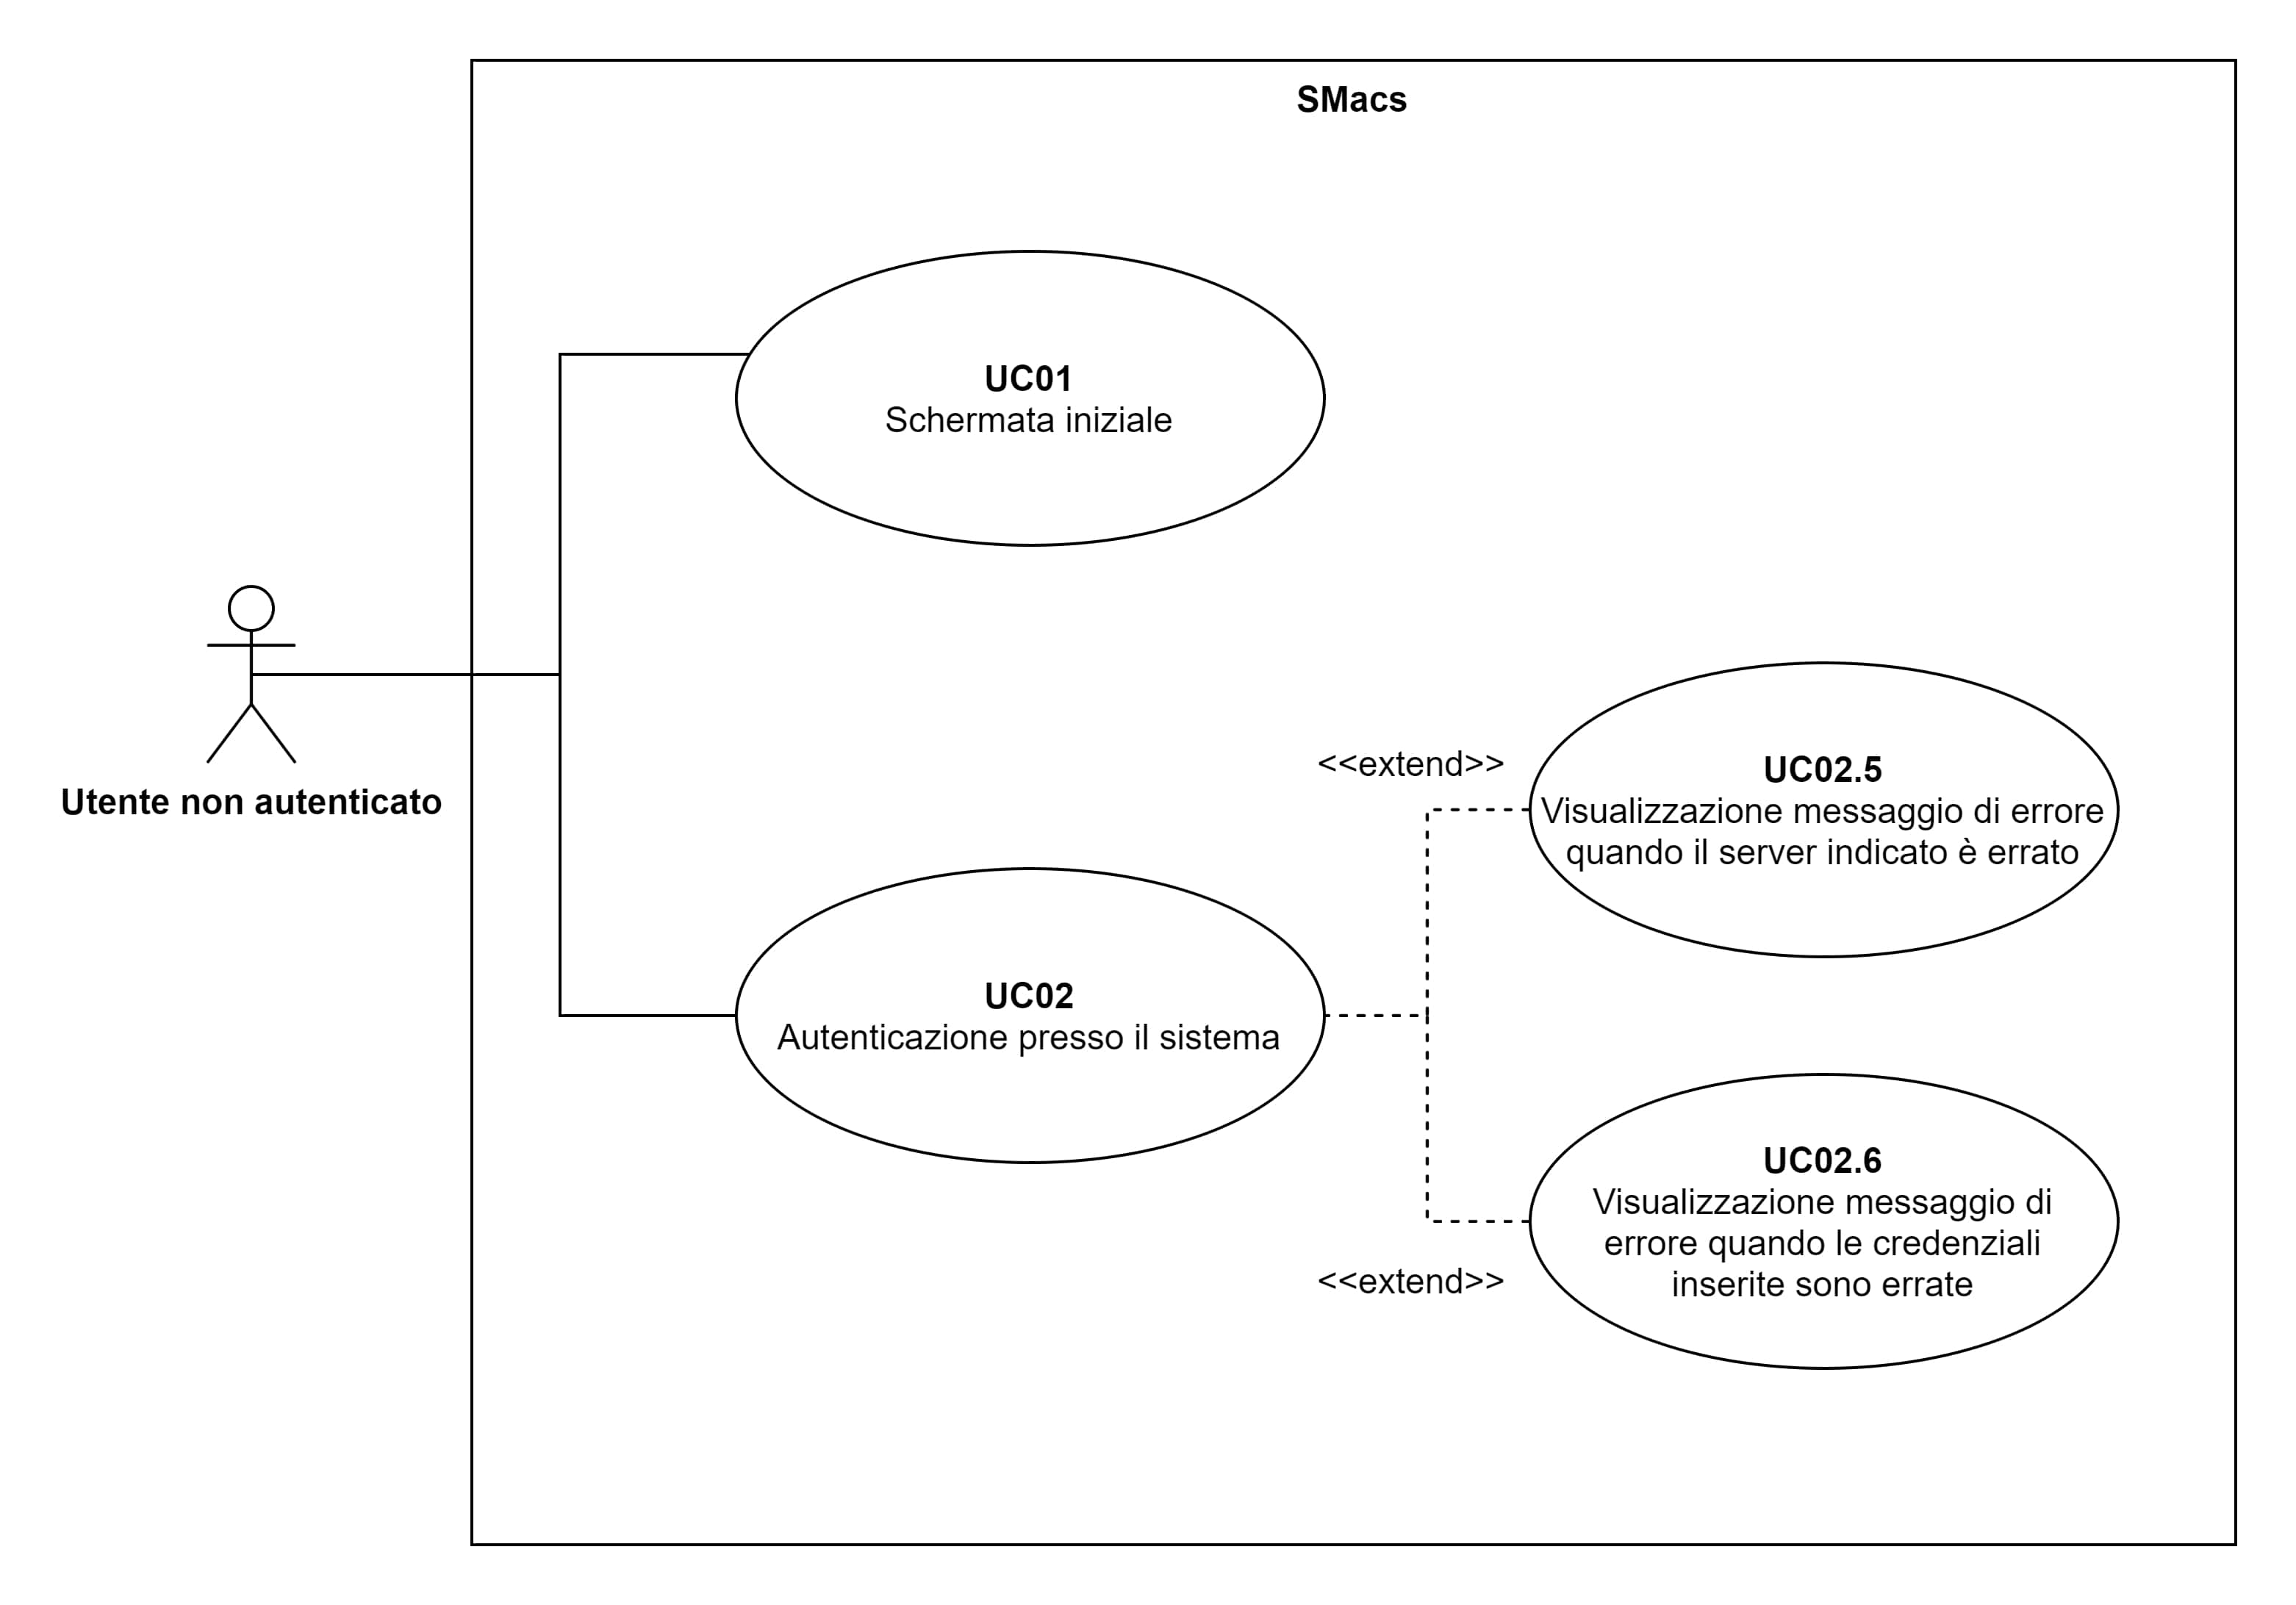
\includegraphics[width=1.0\columnwidth]{appendice-A/utente-non-autenticato} 
    \caption{SMacs - Casi d'uso dell'utente non autenticato}
\end{figure}

\begin{usecase}{01}{Schermata iniziale}
\usecaseprimaryactors{Utente non autenticato}
\usecasepre{L'utente ha appena avviato l'applicazione.}
\usecasedesc{Vengono visualizzati all'utente alcuni link per accedere a vari siti web legati all'azienda e la possibilità di aprire la pagina di accesso alle funzionalità dell'applicazione.}
\usecasepost{Viene visualizzata la schermata iniziale dell'applicazione.}
\label{uc:UC01}
\end{usecase}

\begin{figure}[!h] 
    \centering 
    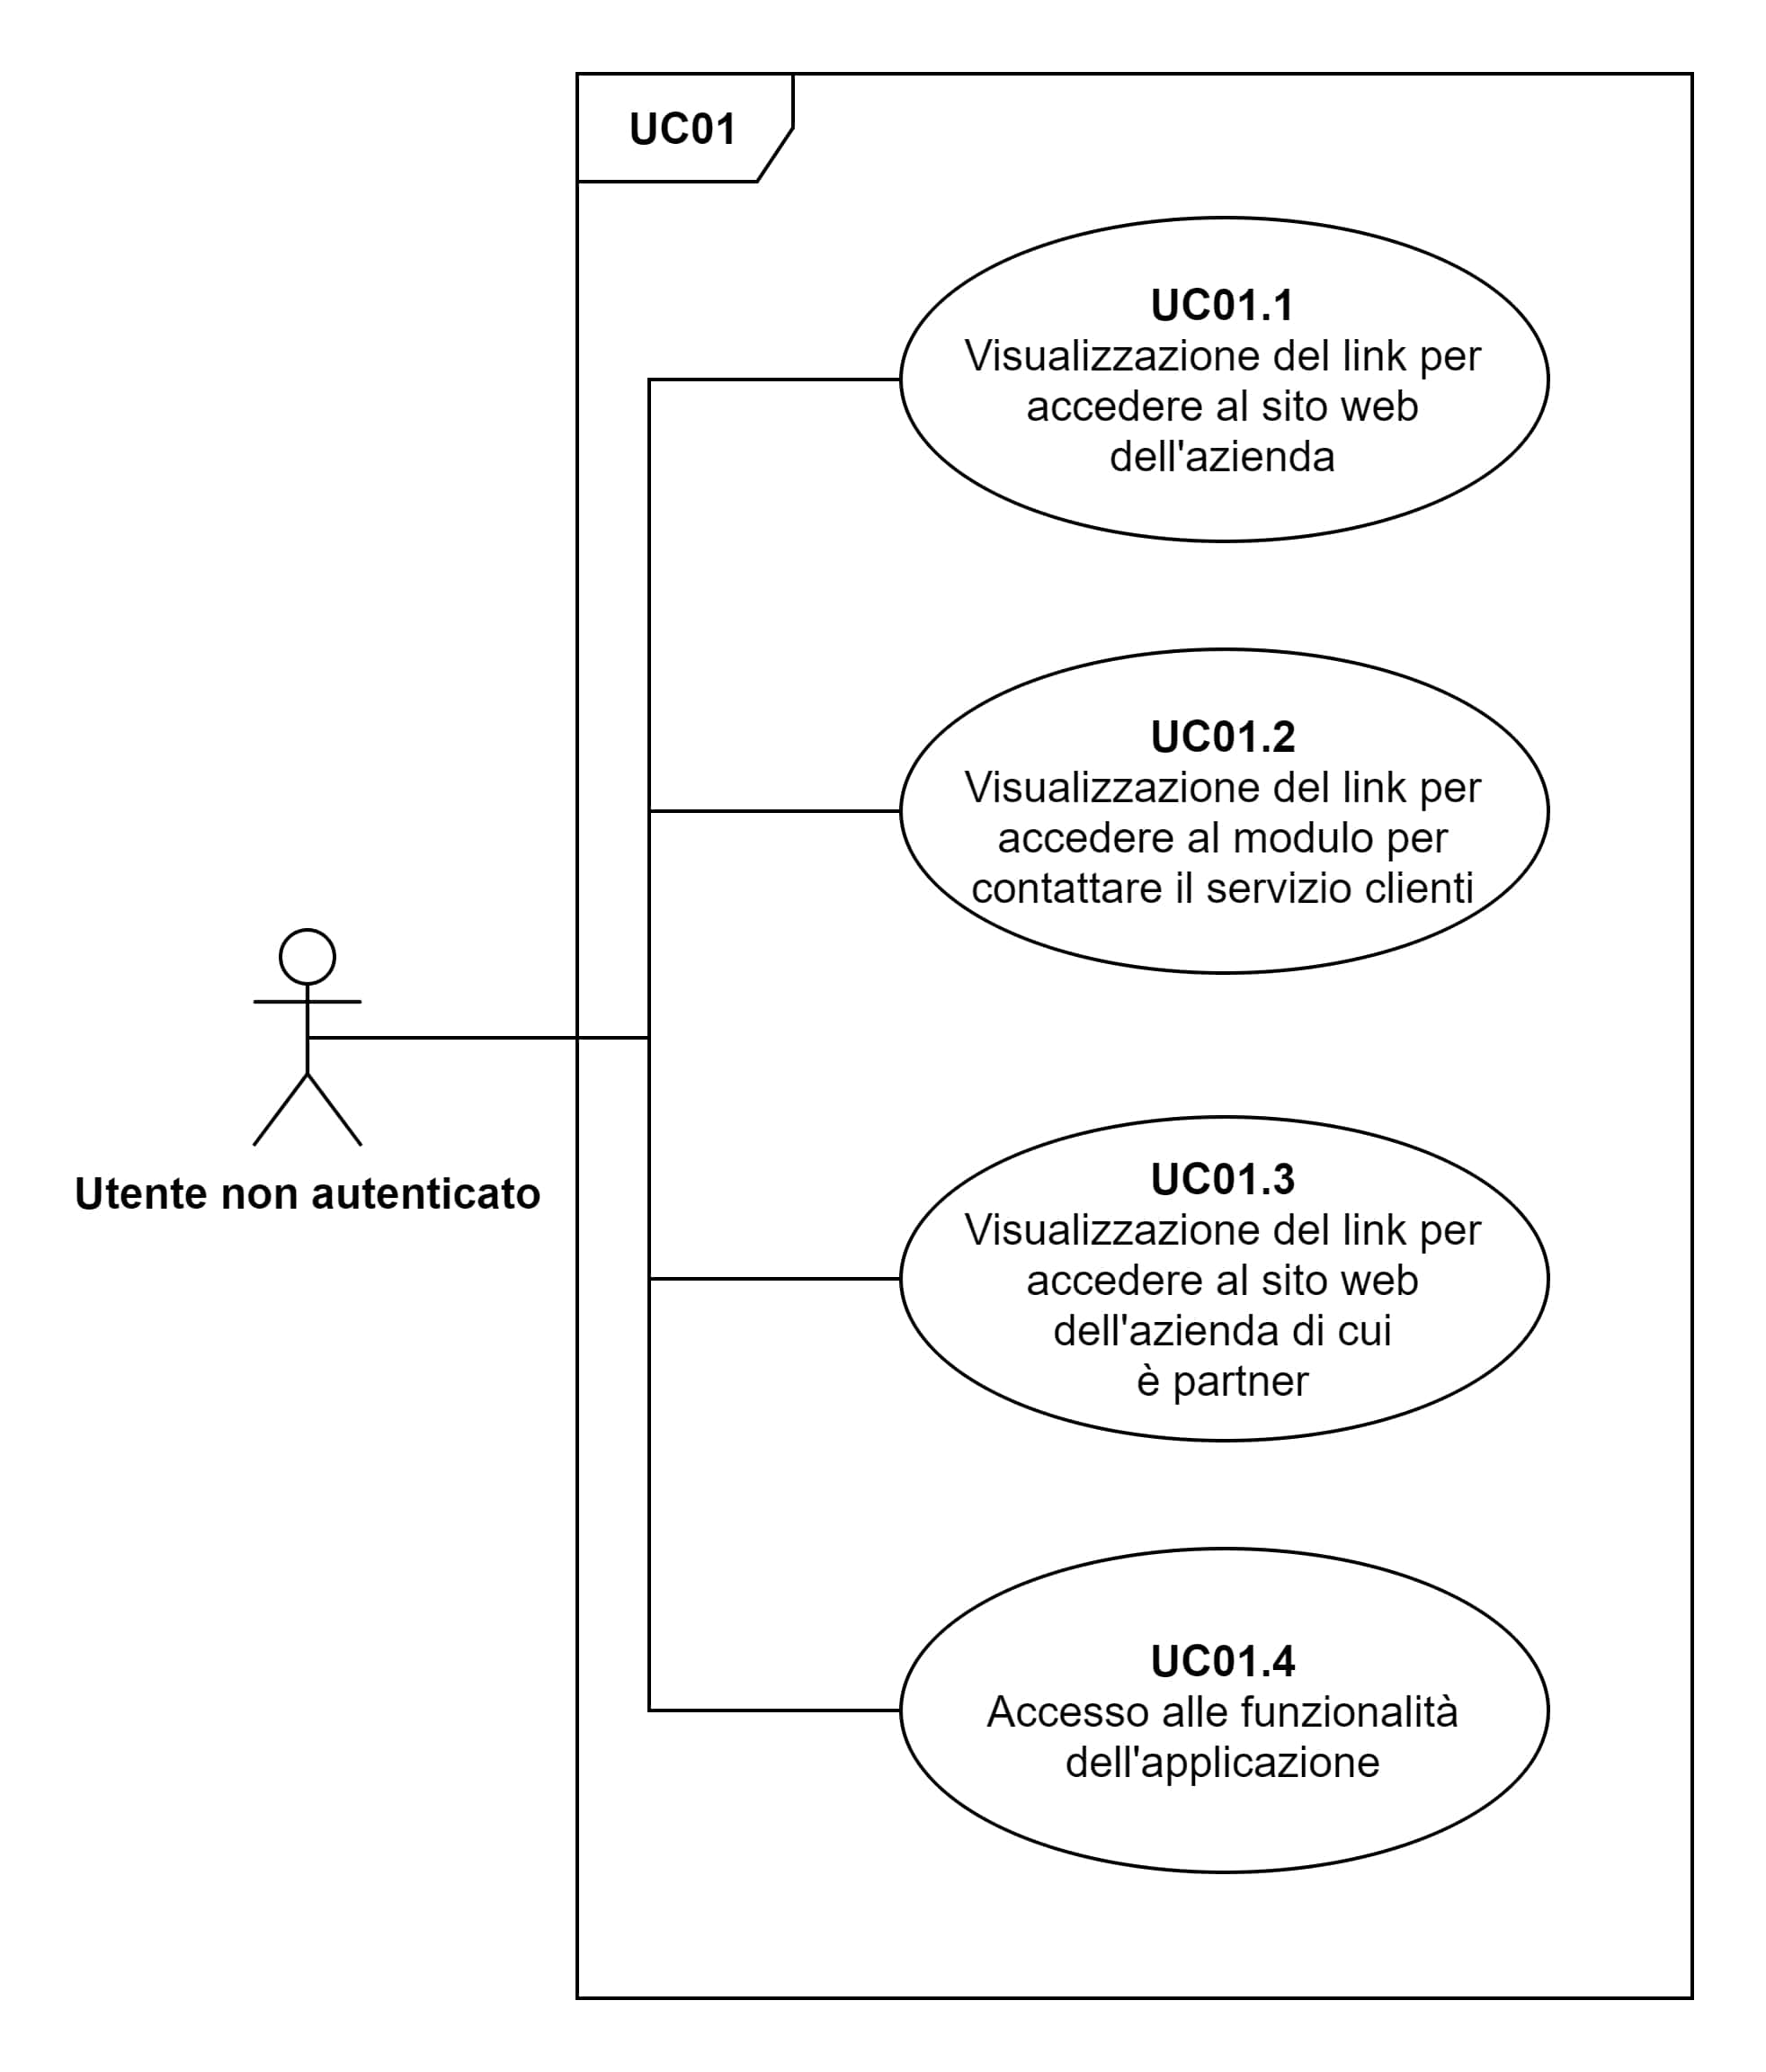
\includegraphics[width=1.0\columnwidth]{appendice-A/uc01} 
    \caption{SMacs - Sotto-casi d'uso di UC01 - Schermata iniziale}
\end{figure}

\begin{usecase}{01.1}{Visualizzazione del link per accedere al sito web dell'azienda}
\usecaseprimaryactors{Utente non autenticato}
\usecasepre{L'utente ha appena avviato l'applicazione.}
\usecasedesc{Viene visualizzato il link per accedere al sito web dell'azienda.}
\usecasepost{Viene visualizzato il link per accedere al sito web dell'azienda.}
\label{uc:UC01-1}
\end{usecase}

\begin{usecase}{01.2}{Visualizzazione del link per accedere al modulo per contattare il servizio clienti}
\usecaseprimaryactors{Utente non autenticato}
\usecasepre{L'utente ha appena avviato l'applicazione.}
\usecasedesc{Viene visualizzato il link per accedere alla pagina web per contattare il servizio clienti.}
\usecasepost{Viene visualizzato il link per accedere al modulo per contattare il servizio clienti.}
\label{uc:UC01-2}
\end{usecase}

\begin{usecase}{01.3}{Visualizzazione del link per accedere al sito web dell'azienda di cui è partner}
\usecaseprimaryactors{Utente non autenticato}
\usecasepre{L'utente ha appena avviato l'applicazione.}
\usecasedesc{Viene visualizzato il link per accedere al sito web dell'azienda di cui è partner.}
\usecasepost{Viene visualizzato il link per accedere al sito web dell'azienda di cui è partner.}
\label{uc:UC01-3}
\end{usecase}

\begin{usecase}{01.4}{Accesso alle funzionalità dell'applicazione}
\usecaseprimaryactors{Utente non autenticato}
\usecasepre{L'utente ha appena avviato l'applicazione.}
\usecasedesc{Viene visualizzato la funzionalità di accesso alla schermata di autenticazione.}
\usecasepost{Viene visualizzato la funzionalità di accesso alla schermata di autenticazione.}
\label{uc:UC01-4}
\end{usecase}

\begin{usecase}{02}{Autenticazione presso il sistema}
\usecaseprimaryactors{Utente non autenticato}
\usecasepre{L'utente ha avviato l'applicazione e ha selezionato la funzionalità di accesso nella schermata iniziale.}
\usecasedesc{L'utente può inserire il server a cui connettersi e le proprie credenziali per poter accedere presso il sistema.}
\usecasepost{L'utente si è autenticato presso il sistema.}
\usecaseext{UC02.5, UC02.6}
\label{uc:UC02}
\end{usecase}

\begin{figure}[!h] 
    \centering 
    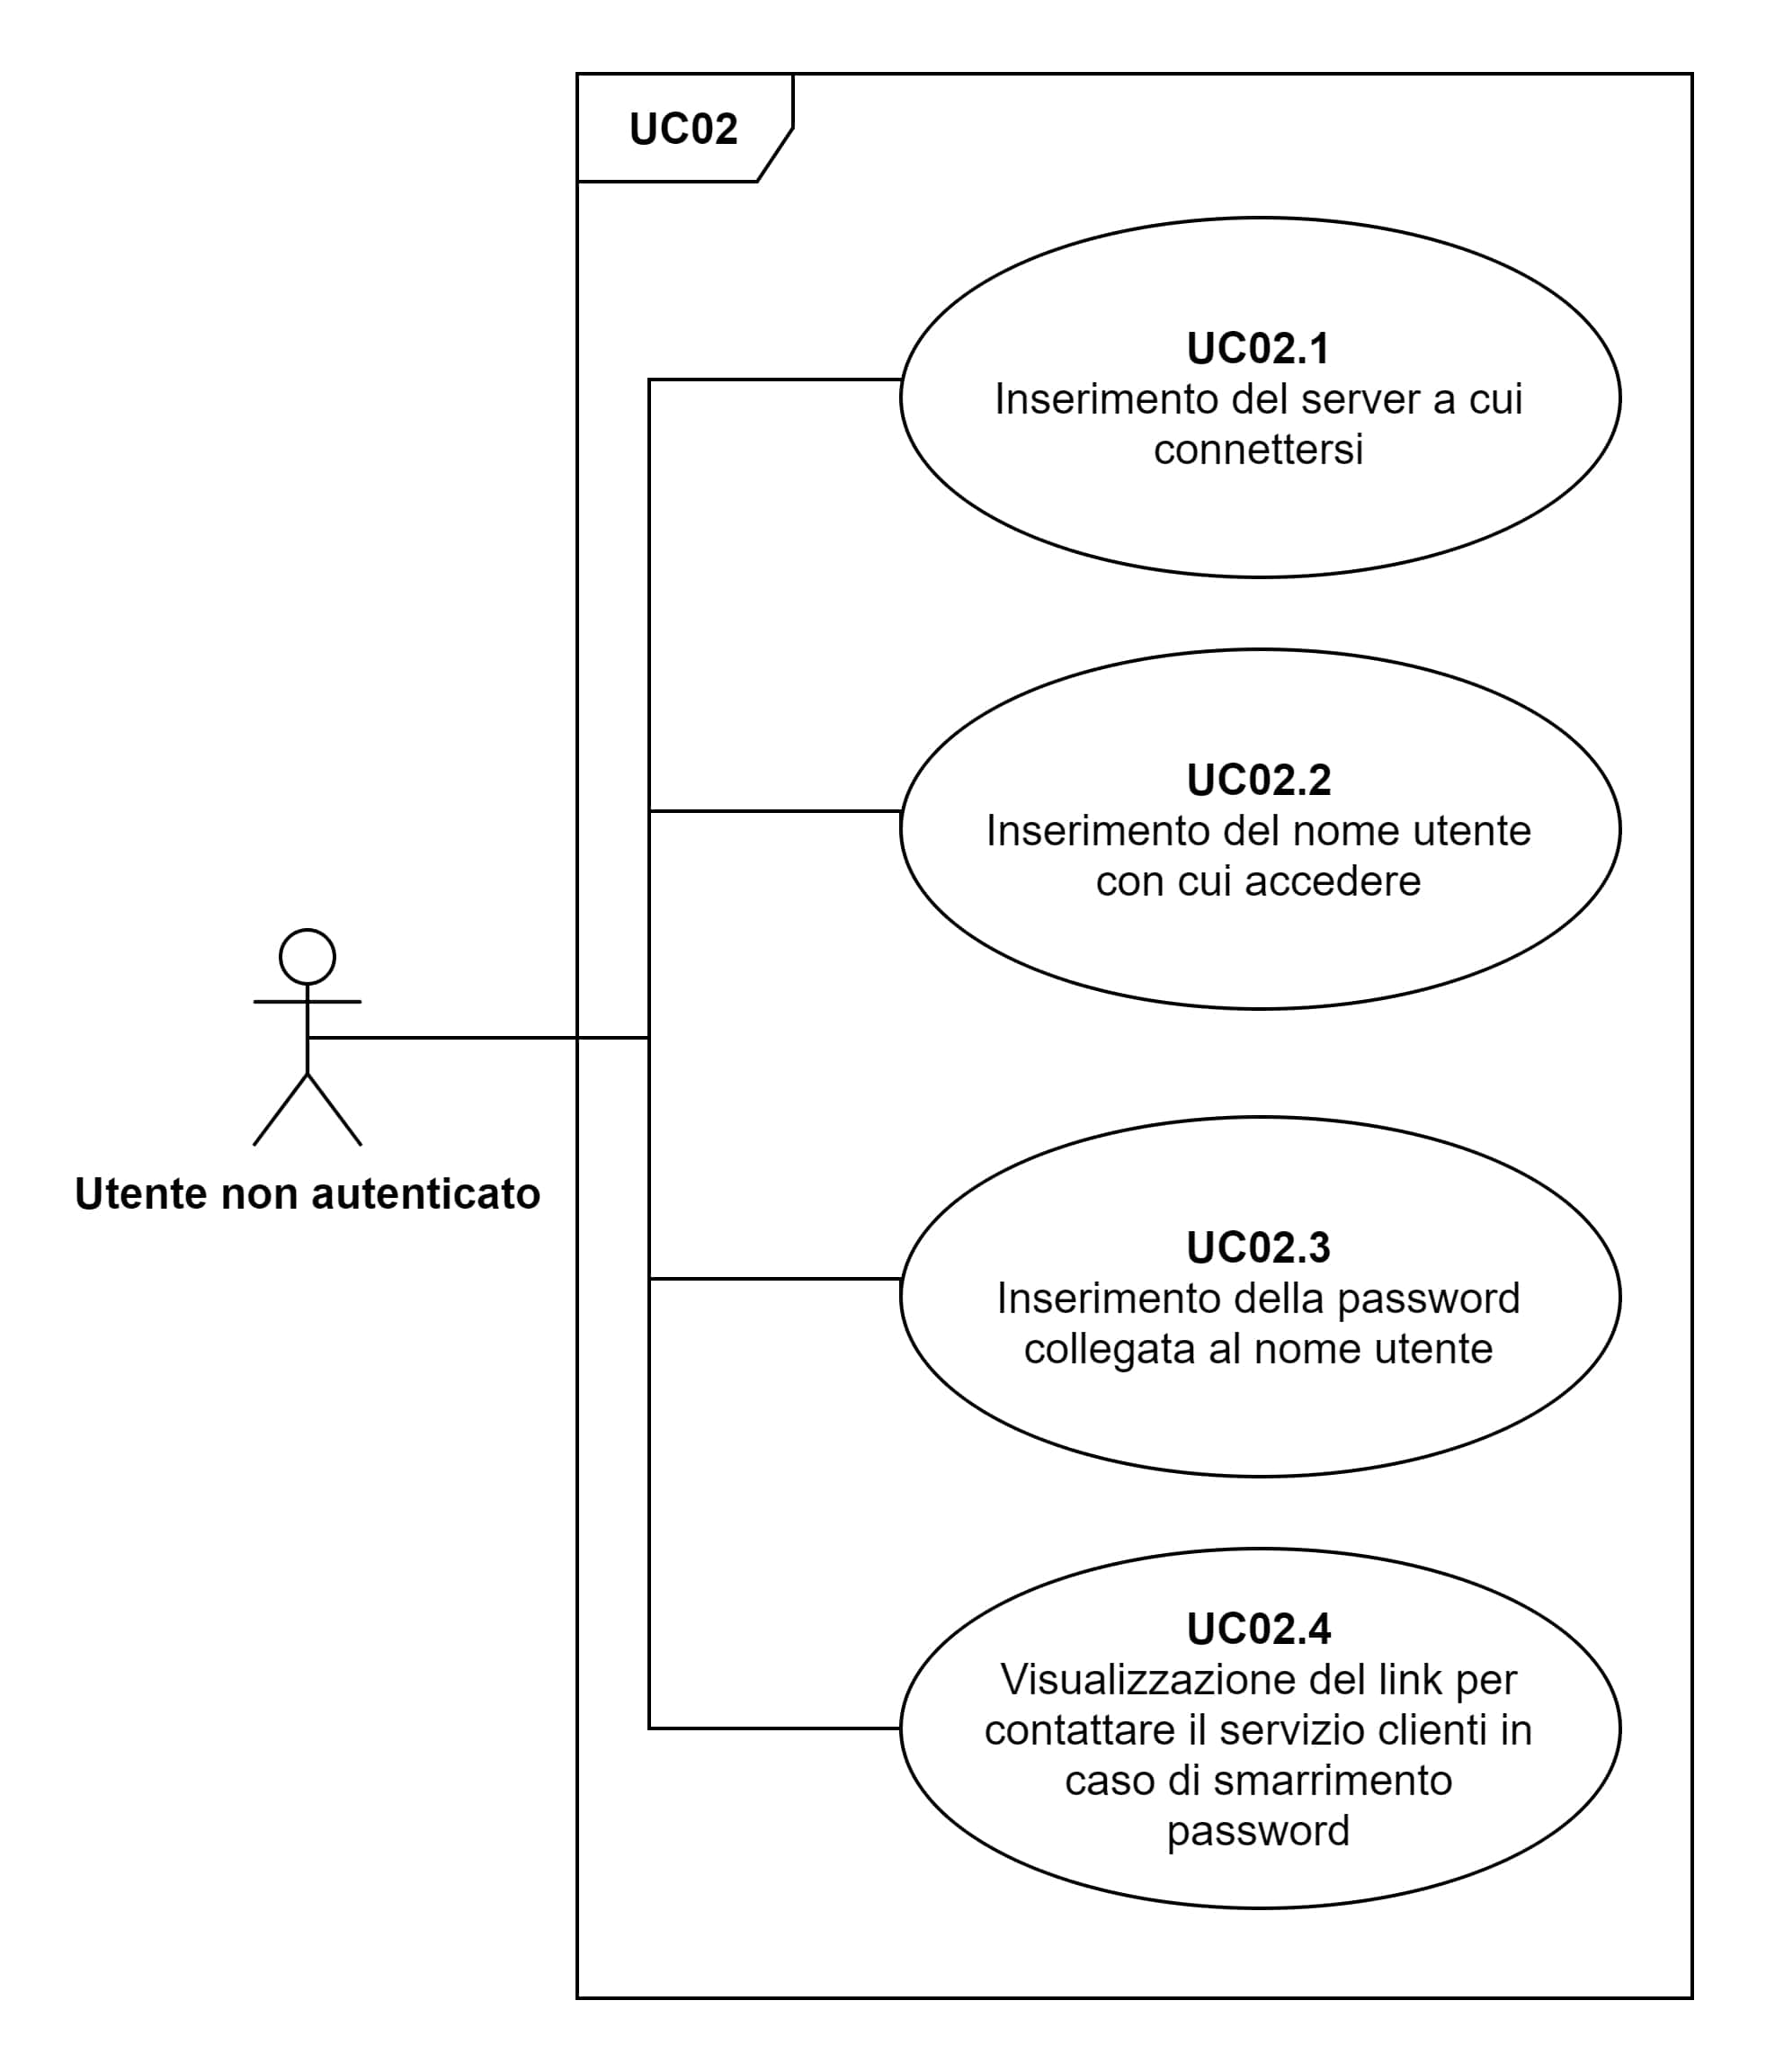
\includegraphics[width=1.0\columnwidth]{appendice-A/uc02} 
    \caption{SMacs - Sotto-casi d'uso di UC02 - Autenticazione presso il sistema}
\end{figure}

\begin{usecase}{02.1}{Inserimento del server a cui connettersi}
\usecaseprimaryactors{Utente non autenticato}
\usecasepre{L'utente ha la possibilità di inserire il server del sistema presso cui connettersi.}
\usecasedesc{L'utente può inserire il server a cui connettersi.}
\usecasepost{L'utente ha inserito il server a cui connettersi.}
\label{uc:UC02-1}
\end{usecase}

\begin{usecase}{02.2}{Inserimento del nome utente con cui accedere}
\usecaseprimaryactors{Utente non autenticato}
\usecasepre{L'utente ha la possibilità di inserire il nome utente con cui connettersi al sistema.}
\usecasedesc{L'utente può inserire il nome utente con cui connettersi al sistema.}
\usecasepost{L'utente ha inserito il proprio nome utente.}
\label{uc:UC02-2}
\end{usecase}

\begin{usecase}{02.3}{Inserimento della password collegata al nome utente}
\usecaseprimaryactors{Utente non autenticato}
\usecasepre{L'utente ha la possibilità di inserire la password con cui connettersi al sistema.}
\usecasedesc{L'utente può inserire la password con cui connettersi al sistema.}
\usecasepost{L'utente ha inserito la propria password.}
\label{uc:UC02-3}
\end{usecase}

\begin{usecase}{02.4}{Visualizzazione del link per contattare il servizio clienti in caso di smarrimento password}
\usecaseprimaryactors{Utente non autenticato}
\usecasepre{L'utente ha la possibilità di contattare il servizio clienti.}
\usecasedesc{L'utente può visualizzare il link per contattare il servizio clienti in caso di smarrimento della password.}
\usecasepost{Viene visualizzato il link per contattare il servizio clienti nel caso di smarrimento della password.}
\label{uc:UC02-4}
\end{usecase}

\begin{usecase}{02.5}{Visualizzazione messaggio di errore quando il server indicato è errato}
\usecaseprimaryactors{Utente non autenticato}
\usecasepre{L'utente ha inserito un server inesistente o a cui non è possibile connettersi.}
\usecasedesc{L'utente ha inserito un server inesistente o a cui non è possibile connettersi, di conseguenza viene visualizzato un messaggio di errore che lo informa del fatto.}
\usecasepost{Viene visualizzato un messaggio di errore che informa l'utente del fatto.}
\label{uc:UC02-5}
\end{usecase}

\begin{usecase}{02.6}{Visualizzazione messaggio di errore quando le credenziali inserite non sono valide}
\usecaseprimaryactors{Utente non autenticato}
\usecasepre{L'utente ha inserito delle credenziali errate.}
\usecasedesc{L'utente ha inserito delle credenziali errate e di conseguenza viene visualizzato un messaggio di errore che lo informa del fatto.}
\usecasepost{Viene visualizzato un messaggio di errore che informa l'utente del fatto.}
\label{uc:UC02-6}
\end{usecase}

% sicurezza che prenda tutto lo spazio disponibile
\clearpage

\begin{figure}[!h] 
    \centering 
    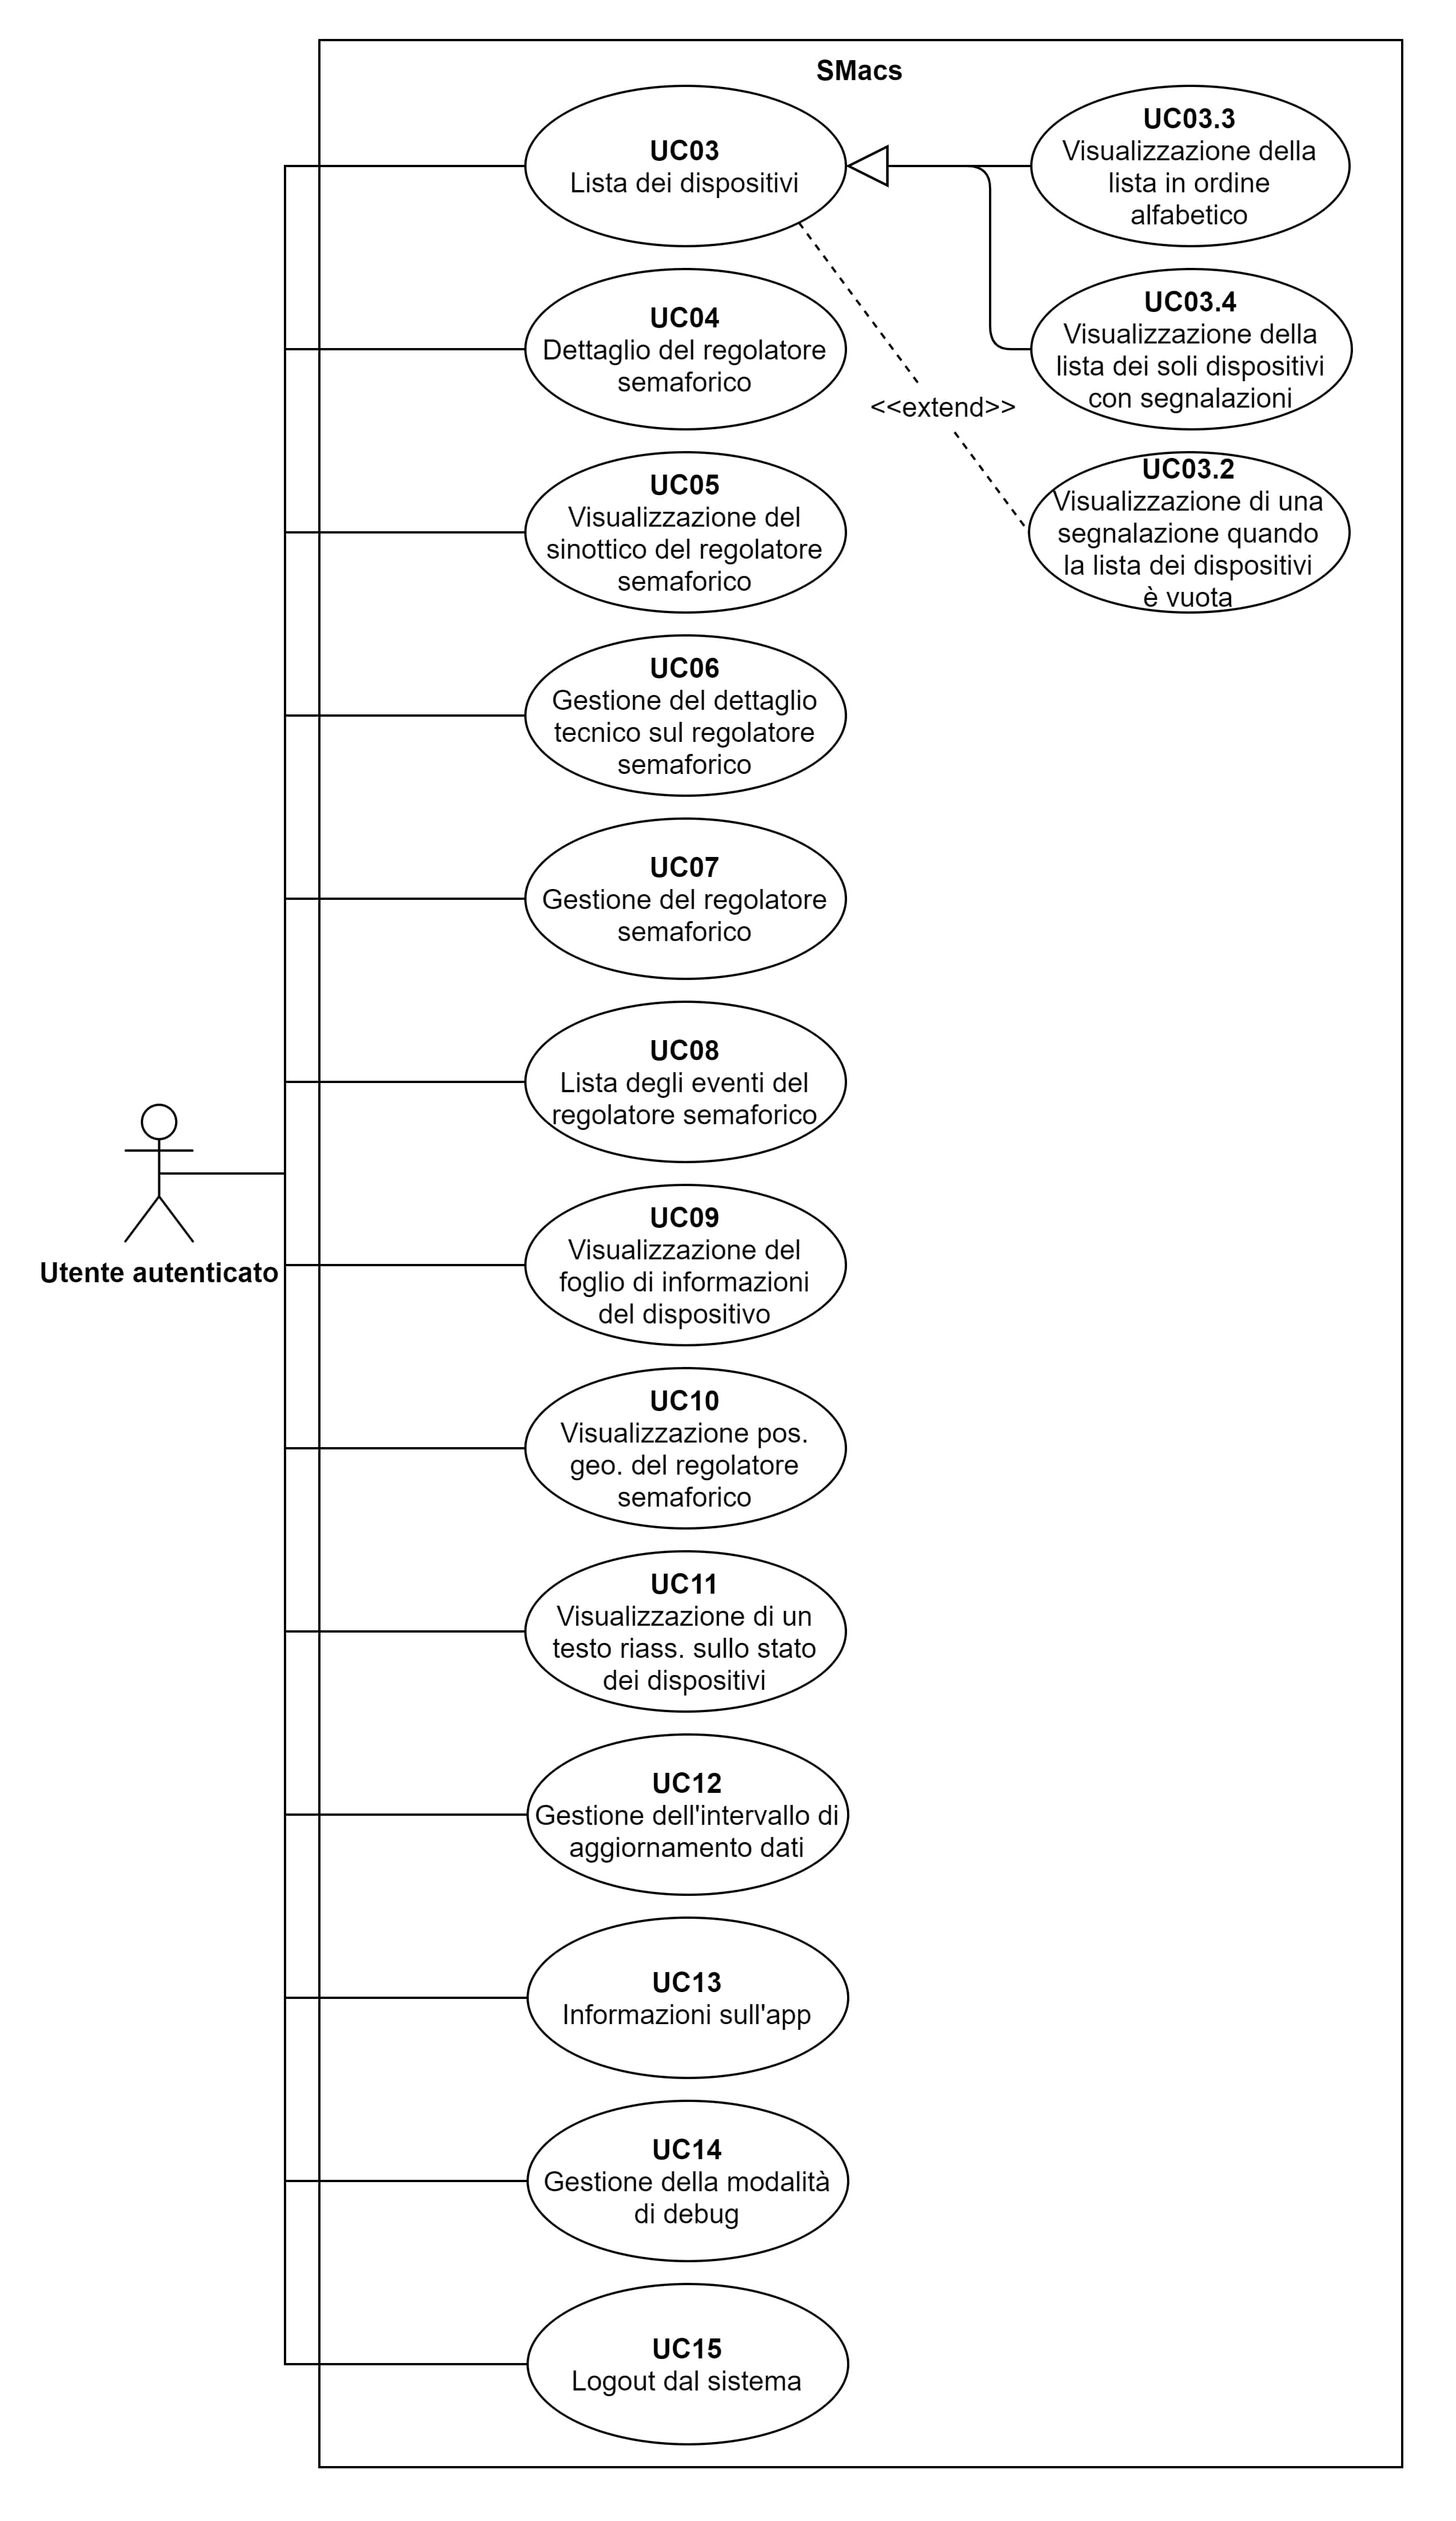
\includegraphics[height=0.94\textheight]{appendice-A/utente-autenticato} 
    \caption{SMacs - Casi d'uso dell'utente autenticato}
\end{figure}

\begin{usecase}{03}{Lista dei dispositivi}
\usecaseprimaryactors{Utente autenticato}
\usecasepre{L'utente ha accesso alla lista dei dispositivi collegati al proprio profilo.}
\usecasedesc{Viene visualizzata la lista dei dispositivi di cui l'utente può avere informazioni a riguardo.}
\usecasepost{Viene visualizzata la lista dei dispositivi di cui l'utente può avere informazioni a riguardo.}
\usecaseext{UC03.2}
\label{uc:UC03}
\end{usecase}

\begin{figure}[!h] 
    \centering 
    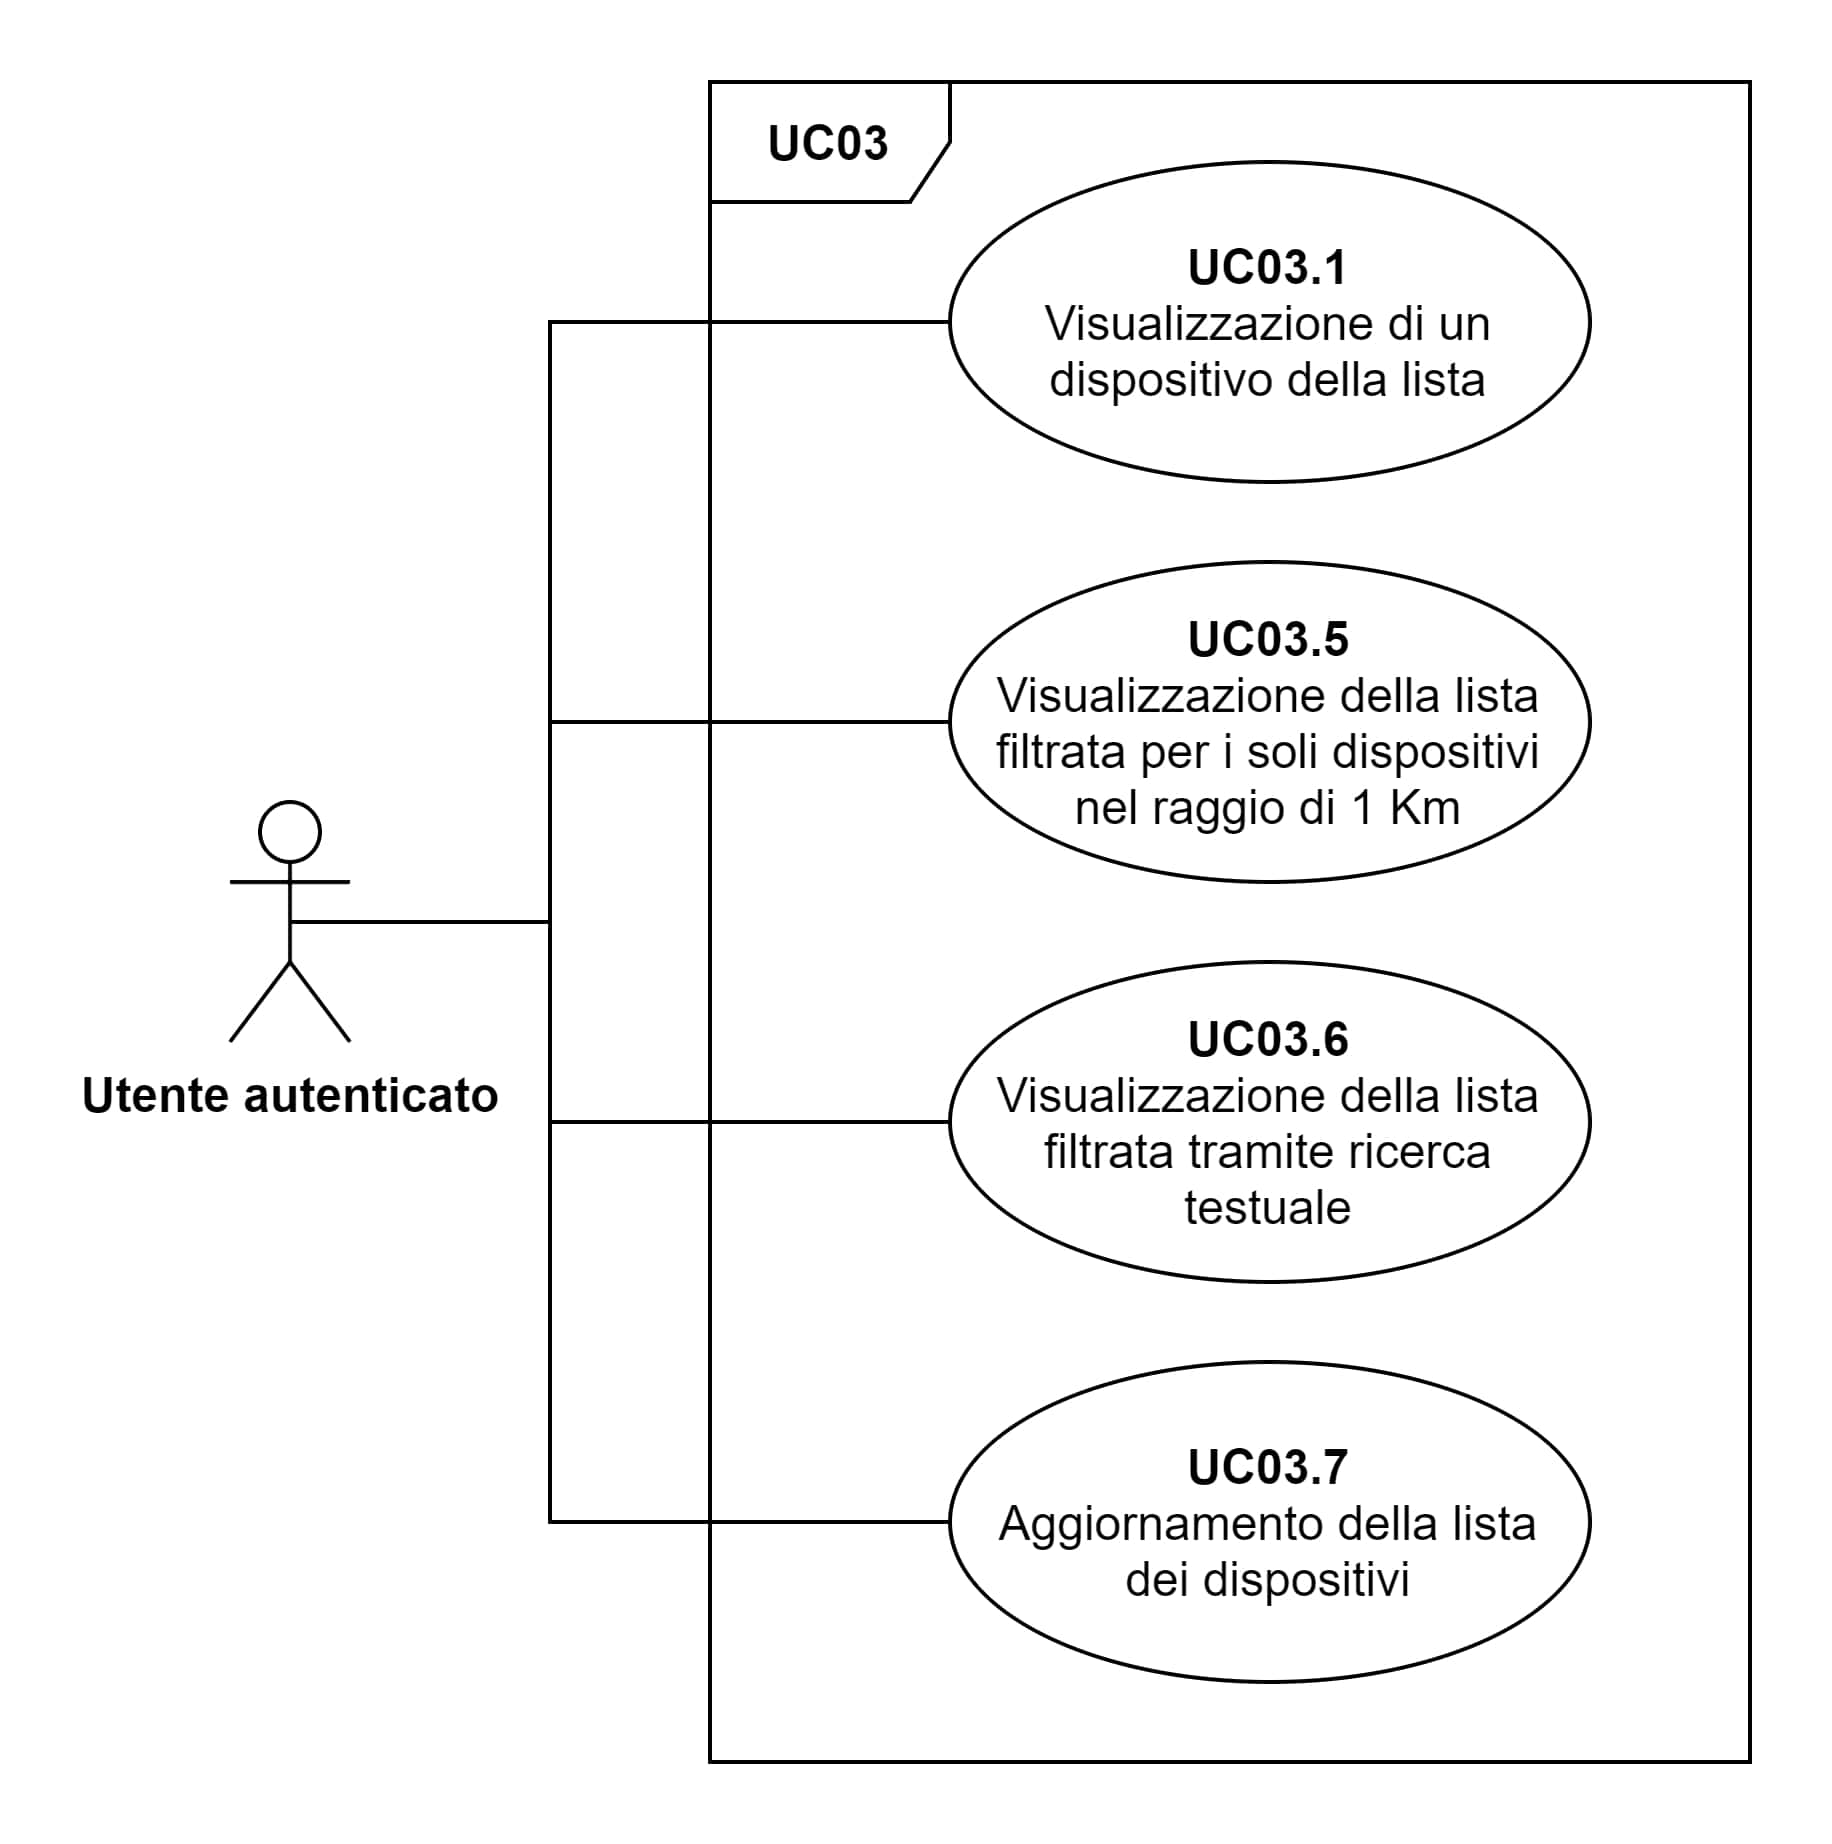
\includegraphics[width=1.0\columnwidth]{appendice-A/uc03} 
    \caption{SMacs - Sotto-casi d'uso di UC03 - Lista dei dispositivi}
\end{figure}

\begin{usecase}{03.1}{Visualizzazione di un dispositivo della lista}
\usecaseprimaryactors{Utente autenticato}
\usecasepre{L'utente sta visionando la lista dei dispositivi collegati al proprio profilo.}
\usecasedesc{Viene visualizzato un dispositivo della lista dei dispositivi collegati al profilo dell'utente, mostrandone un'icona rappresentativa e un dettaglio compatto che comprende il codice, il nome, lo stato attuale e il livello massimo di segnalazione attuale. Inoltre, viene mostrata la data di ultimo aggiornamento.}
\usecasepost{Viene visualizzato un dispositivo della lista dei dispositivi collegati al profilo dell'utente, mostrandone un dettaglio compatto.}
\label{uc:UC03-1}
\end{usecase}

\begin{usecase}{03.2}{Visualizzazione di una segnalazione quando la lista dei dispositivi è vuota}
\usecaseprimaryactors{Utente autenticato}
\usecasepre{L'utente sta visionando la lista dei dispositivi collegati al proprio profilo ma è vuota.}
\usecasedesc{L'utente sta visionando la lista dei dispositivi collegati al proprio profilo ma è vuota, quindi viene avvisato mediante un messaggio,}
\usecasepost{Viene visualizzato un messaggio che avvisa l'utente che la lista è vuota.}
\label{uc:UC03-2}
\end{usecase}

\begin{usecase}{03.3}{Visualizzazione della lista in ordine alfabetico}
\usecaseprimaryactors{Utente autenticato}
\usecasepre{L'utente sta visionando la lista dei dispositivi collegati al proprio profilo.}
\usecasedesc{Viene visualizzata la lista dei dispositivi di cui l'utente può avere informazioni a riguardo in ordine alfabetico (corrisponde all'opzione di default).}
\usecasepost{Viene visualizzata la lista dei dispositivi di cui l'utente può avere informazioni a riguardo in ordine alfabetico.}
\usecasegen{UC03}
\label{uc:UC03-3}
\end{usecase}

\begin{usecase}{03.4}{Visualizzazione della lista dei soli dispositivi con segnalazioni}
\usecaseprimaryactors{Utente autenticato}
\usecasepre{L'utente sta visionando la lista dei dispositivi collegati al proprio profilo.}
\usecasedesc{Viene visualizzata la lista dei dispositivi con segnalazioni (di malfunzionamento) di cui l'utente può avere informazioni a riguardo.}
\usecasepost{Viene visualizzata la lista dei dispositivi con segnalazioni (di malfunzionamento) di cui l'utente può avere informazioni a riguardo.}
\usecasegen{UC03}
\label{uc:UC03-4}
\end{usecase}

\begin{usecase}{03.5}{Visualizzazione della lista filtrata per i soli dispositivi nel raggio di 1 Km}
\usecaseprimaryactors{Utente autenticato}
\usecasepre{L'utente sta visionando la lista dei dispositivi collegati al proprio profilo.}
\usecasedesc{Viene visualizzata la lista dei dispositivi entro il raggio di 1 Km dalla posizione geografica attuale dell'utente di cui l'utente può avere informazioni a riguardo.}
\usecasepost{Viene visualizzata la lista dei dispositivi entro il raggio di 1 Km dalla posizione geografica attuale dell'utente di cui l'utente può avere informazioni a riguardo.}
\label{uc:UC03-5}
\end{usecase}

\begin{usecase}{03.6}{Visualizzazione della lista filtrata tramite ricerca testuale}
\usecaseprimaryactors{Utente autenticato}
\usecasepre{L'utente sta visionando la lista dei dispositivi collegati al proprio profilo.}
\usecasedesc{Viene visualizzata la lista dei dispositivi in base alla ricerca inoltrata di cui l'utente può avere informazioni a riguardo.}
\usecasepost{Viene visualizzata la lista dei dispositivi in base alla ricerca inoltrata di cui l'utente può avere informazioni a riguardo.}
\label{uc:UC03-6}
\end{usecase}

\begin{usecase}{03.7}{Aggiornamento della lista dei dispositivi}
\usecaseprimaryactors{Utente autenticato}
\usecasepre{L'utente sta visionando la lista dei dispositivi collegati al proprio profilo.}
\usecasedesc{L'utente seleziona la funzionalità di aggiornamento e viene aggiornata la lista dei dispositivi di cui l'utente può avere informazioni a riguardo ottenendone una nuova copia dal sistema.}
\usecasepost{L'utente seleziona la funzionalità di aggiornamento e viene aggiornata la lista dei dispositivi di cui l'utente può avere informazioni a riguardo ottenendone una nuova copia dal sistema.}
\label{uc:UC03-7}
\end{usecase}

\begin{usecase}{04}{Dettaglio del regolatore semaforico}
\usecaseprimaryactors{Utente autenticato}
\usecasepre{L'utente sta visionando la lista dei dispositivi collegati al proprio profilo e seleziona un regolatore semaforico dalla lista.}
\usecasedesc{Vengono visualizzati informazioni dettagliate sullo stato del regolatore semaforico.}
\usecasepost{Vengono visualizzati informazioni dettagliate sullo stato del regolatore semaforico.}
\label{uc:UC04}
\end{usecase}

\begin{figure}[!h] 
    \centering 
    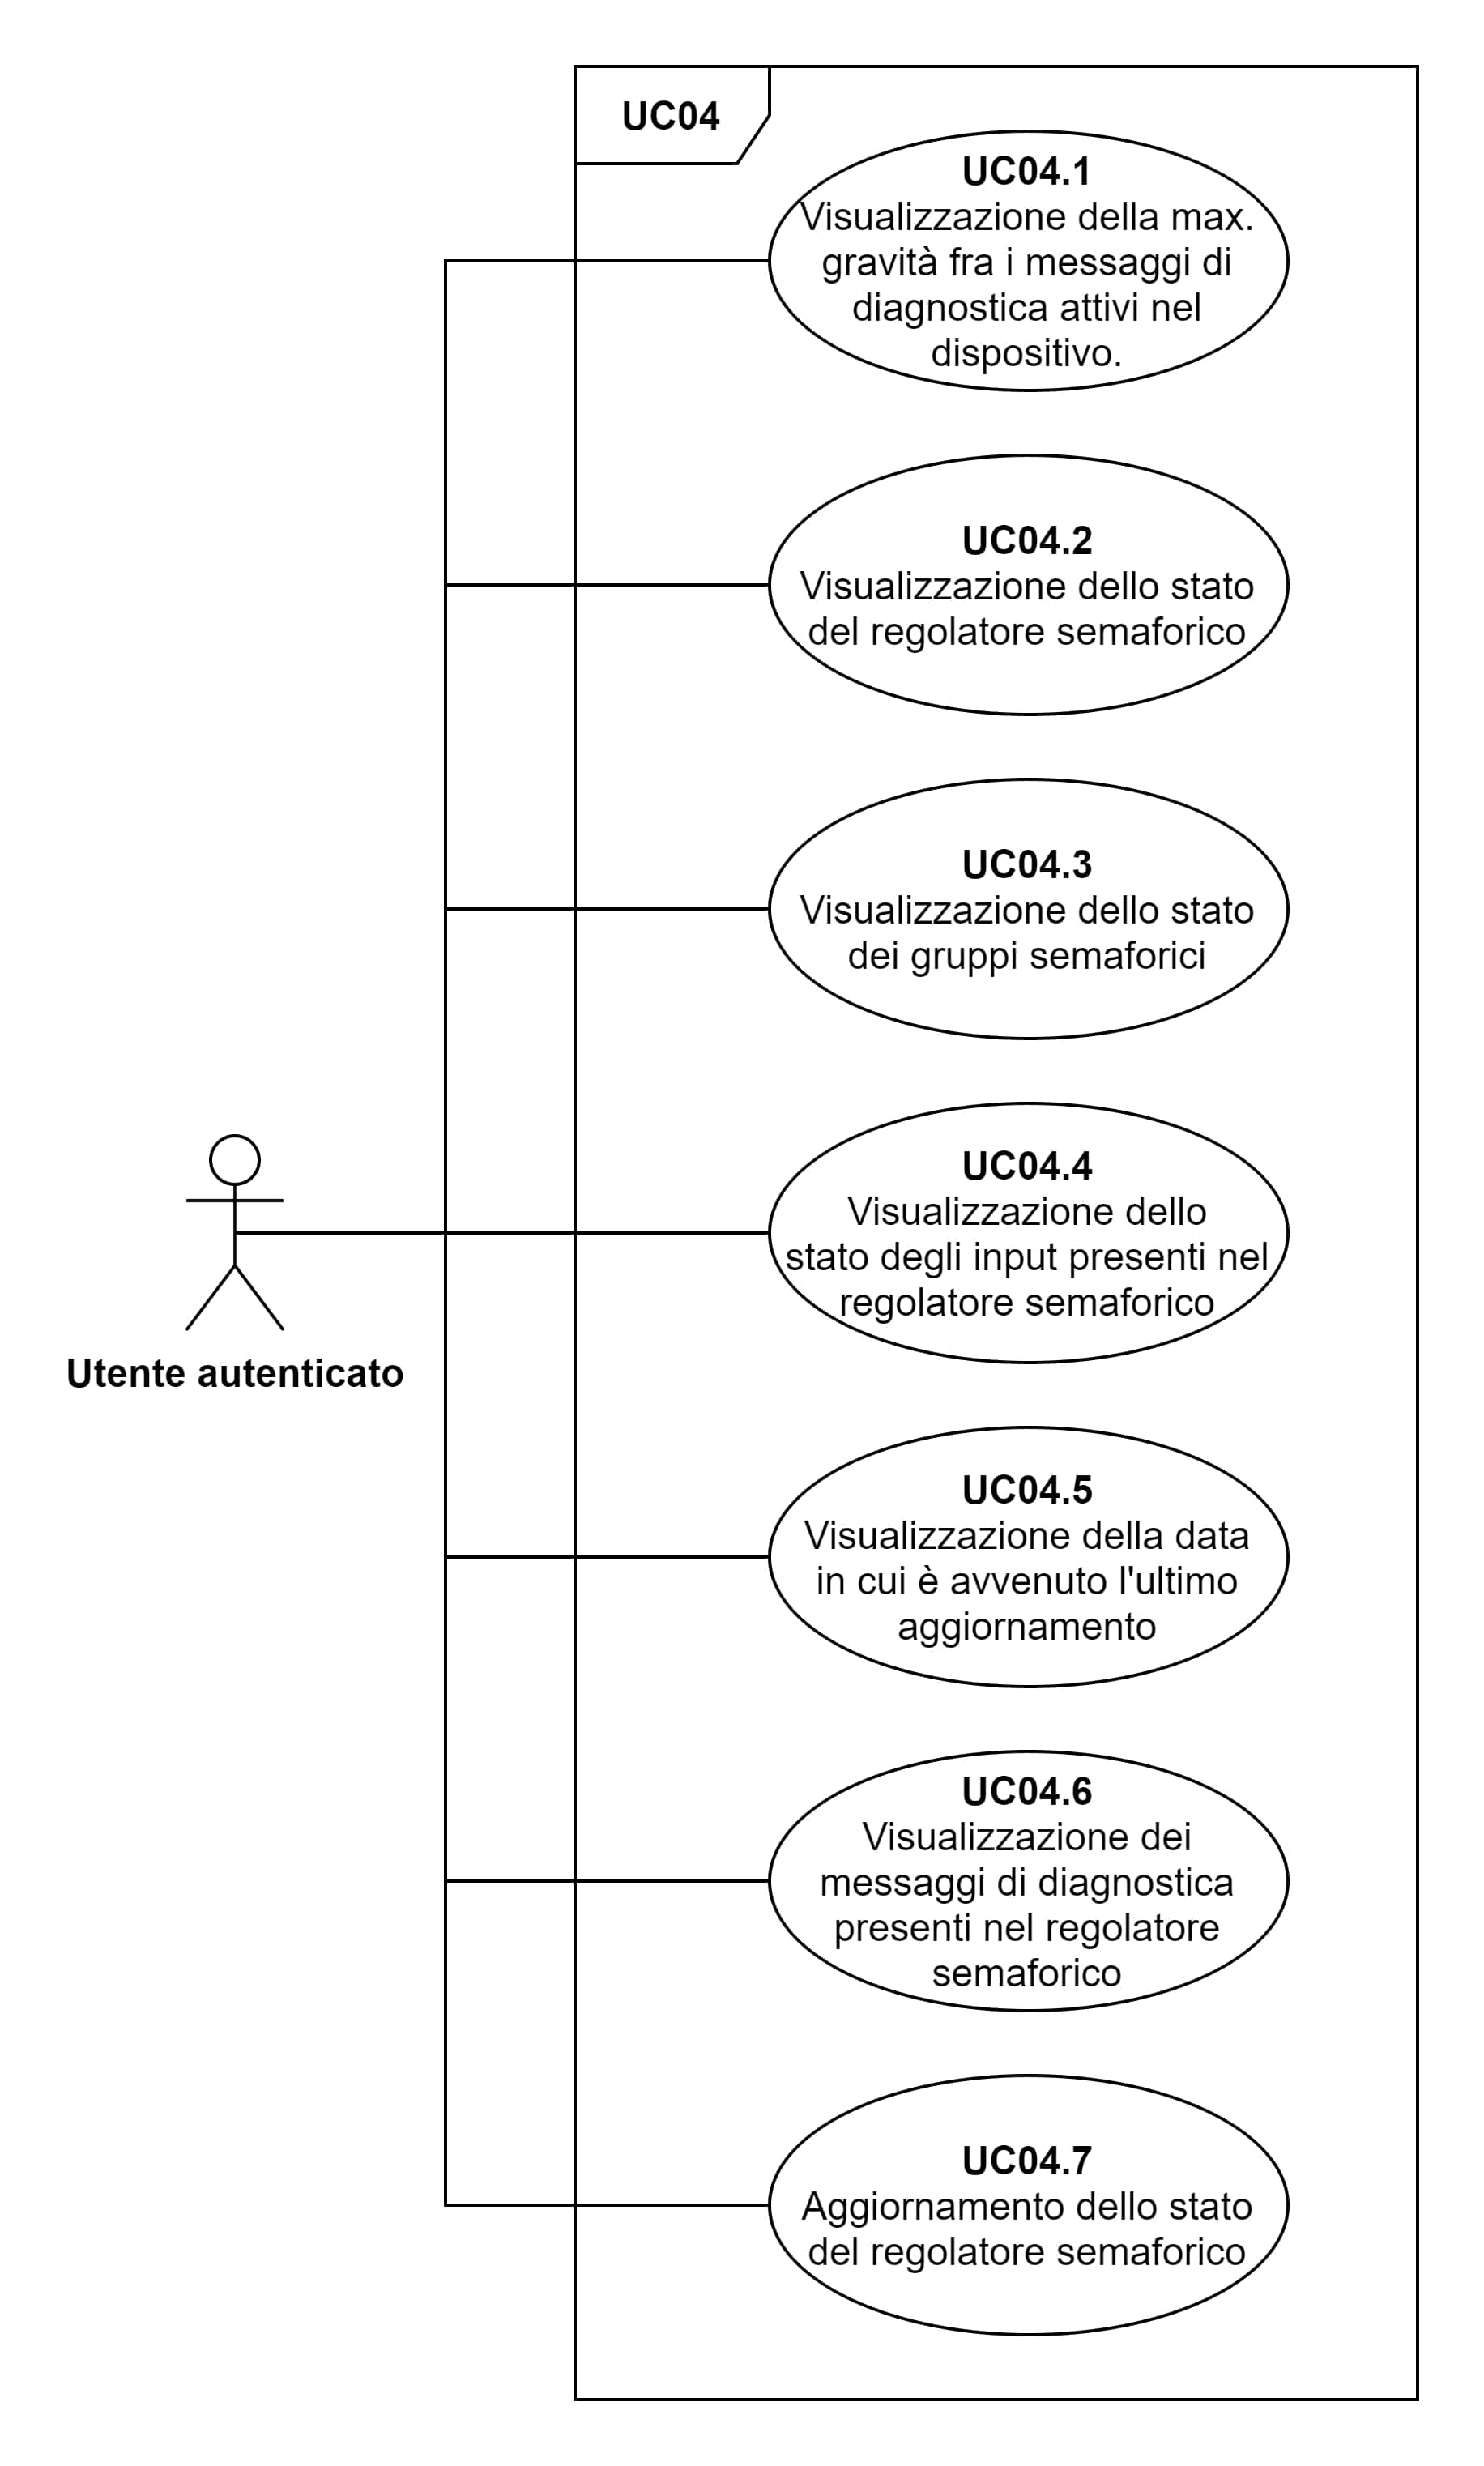
\includegraphics[width=0.9\columnwidth]{appendice-A/uc04} 
    \caption{SMacs - Sotto-casi d'uso di UC04 - Dettaglio del regolatore semaforico}
\end{figure}

\begin{usecase}{04.1}{Visualizzazione della massima gravità fra i messaggi di diagnostica attivi nel dispositivo.}
\usecaseprimaryactors{Utente autenticato}
\usecasepre{L'utente sta visionando il dettaglio del regolatore semaforico selezionato dalla lista.}
\usecasedesc{Viene visualizzato lo stato di diagnostica del regolatore semaforico.}
\usecasepost{Viene visualizzato lo stato di diagnostica del regolatore semaforico.}
\label{uc:UC04-1}
\end{usecase}

\begin{usecase}{04.2}{Visualizzazione dello stato del regolatore semaforico}
\usecaseprimaryactors{Utente autenticato}
\usecasepre{L'utente sta visionando il dettaglio del regolatore semaforico selezionato dalla lista.}
\usecasedesc{Viene visualizzato lo stato del regolatore semaforico (funzione, modalità, livello, step, tempo).}
\usecasepost{Viene visualizzato lo stato del regolatore semaforico (funzione, modalità, livello, step, tempo).}
\label{uc:UC04-2}
\end{usecase}

\begin{usecase}{04.3}{Visualizzazione dello stato dei gruppi semaforici}
\usecaseprimaryactors{Utente autenticato}
\usecasepre{L'utente sta visionando il dettaglio del regolatore semaforico selezionato dalla lista.}
\usecasedesc{Viene visualizzato lo stato dei gruppi semaforici.}
\usecasepost{Viene visualizzato lo stato dei gruppi semaforici.}
\label{uc:UC04-3}
\end{usecase}

\begin{usecase}{04.4}{Visualizzazione dello stato degli input presenti nel regolatore semaforico}
\usecaseprimaryactors{Utente autenticato}
\usecasepre{L'utente sta visionando il dettaglio del regolatore semaforico selezionato dalla lista.}
\usecasedesc{Viene visualizzato lo stato degli input presenti nel regolatore semaforico.}
\usecasepost{Viene visualizzato lo stato degli input presenti nel regolatore semaforico.}
\label{uc:UC04-4}
\end{usecase}

\begin{usecase}{04.5}{Visualizzazione della data in cui è avvenuto l'ultimo aggiornamento}
\usecaseprimaryactors{Utente autenticato}
\usecasepre{L'utente sta visionando il dettaglio del regolatore semaforico selezionato dalla lista.}
\usecasedesc{Viene visualizzata la data dell'ultimo aggiornamento del dettaglio del regolatore semaforico.}
\usecasepost{Viene visualizzata la data dell'ultimo aggiornamento del dettaglio del regolatore semaforico.}
\label{uc:UC04-5}
\end{usecase}

\begin{usecase}{04.6}{Visualizzazione dei messaggi di diagnostica presenti nel regolatore semaforico}
\usecaseprimaryactors{Utente autenticato}
\usecasepre{L'utente sta visionando il dettaglio del regolatore semaforico selezionato dalla lista.}
\usecasedesc{Vengono visualizzati i messaggi di diagnostica presenti nel regolatore semaforico.}
\usecasepost{Vengono visualizzati i messaggi di diagnostica presenti nel regolatore semaforico.}
\label{uc:UC04-6}
\end{usecase}

\begin{usecase}{04.7}{Aggiornamento dello stato del regolatore semaforico}
\usecaseprimaryactors{Utente autenticato}
\usecasepre{L'utente sta visionando il dettaglio del regolatore semaforico selezionato dalla lista.}
\usecasedesc{L'utente seleziona la funzionalità di aggiornamento e viene aggiornato lo stato del regolatore semaforico.}
\usecasepost{L'utente seleziona la funzionalità di aggiornamento e viene aggiornato lo stato del regolatore semaforico.}
\label{uc:UC04-7}
\end{usecase}

\begin{usecase}{05}{Visualizzazione del sinottico del regolatore semaforico}
\usecaseprimaryactors{Utente autenticato}
\usecasepre{L'utente sta visionando il dettaglio del regolatore semaforico selezionato dalla lista.}
\usecasedesc{L'utente ha selezionato la funzionalità di visualizzazione del sinottico del regolatore semaforico.}
\usecasepost{L'utente ha selezionato la funzionalità di visualizzazione del sinottico del regolatore semaforico, che presenta una vista d'insieme del tratto di strada in cui è posizionato il regolatore semaforico.}
\label{uc:UC05}
\end{usecase}

\begin{usecase}{06}{Gestione del dettaglio tecnico sul regolatore semaforico}
\usecaseprimaryactors{Utente autenticato}
\usecasepre{L'utente sta visionando il dettaglio del regolatore semaforico selezionato dalla lista.}
\usecasedesc{L'utente può gestire il dettaglio tecnico del regolatore semaforico, visualizzandolo e aggiungendo note.}
\usecasepost{L'utente può gestire il dettaglio tecnico del regolatore semaforico, visualizzandolo e aggiungendo note.}
\label{uc:UC06}
\end{usecase}

\begin{figure}[!h] 
    \centering 
    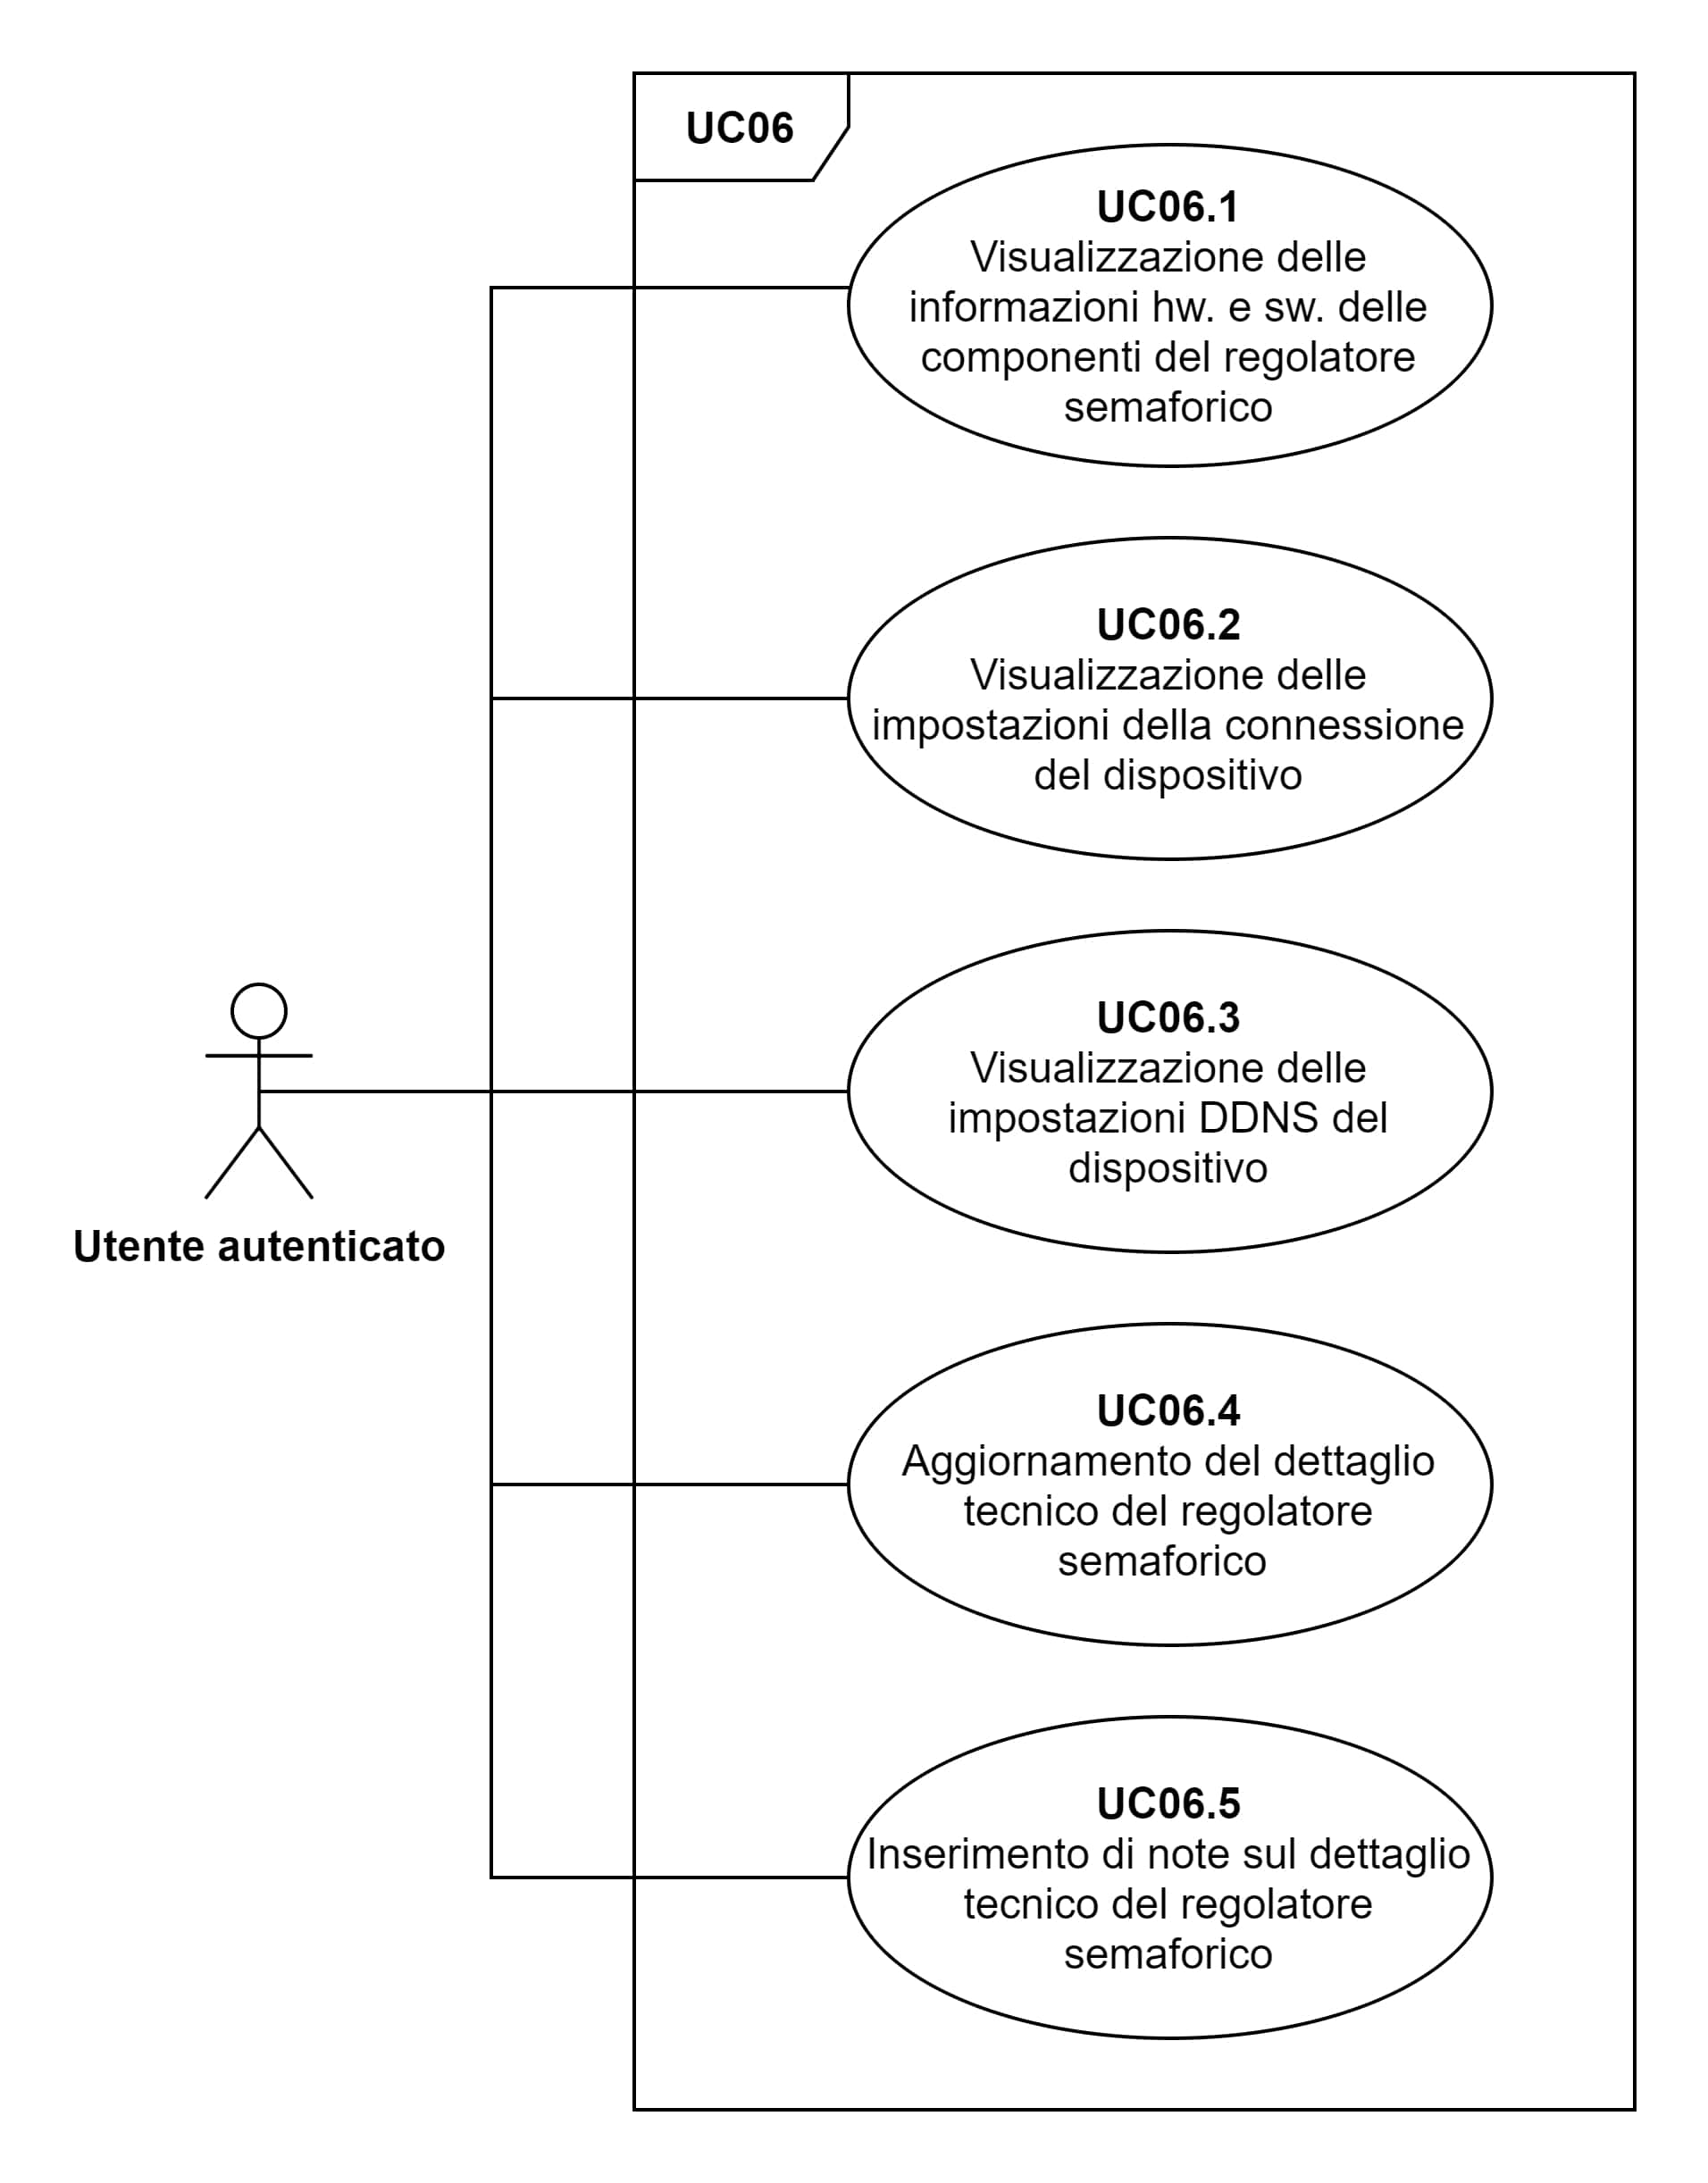
\includegraphics[width=1.0\columnwidth]{appendice-A/uc06} 
    \caption{SMacs - Sotto-casi d'uso di UC06 - Gestione del dettaglio tecnico sul regolatore semaforico}
\end{figure}

\begin{usecase}{06.1}{Visualizzazione delle informazioni hardware e software delle componenti del regolatore semaforico}
\usecaseprimaryactors{Utente autenticato}
\usecasepre{L'utente sta visionando il dettaglio tecnico del regolatore semaforico.}
\usecasedesc{Vengono visualizzate le informazioni hardware e software delle componenti del regolatore semaforico.}
\usecasepost{Vengono visualizzate le informazioni hardware e software delle componenti del regolatore semaforico.}
\label{uc:UC06-1}
\end{usecase}

\begin{usecase}{06.2}{Visualizzazione delle impostazioni della connessione del dispositivo}
\usecaseprimaryactors{Utente autenticato}
\usecasepre{L'utente sta visionando il dettaglio tecnico del regolatore semaforico.}
\usecasedesc{Vengono visualizzati l'indirizzo IP e la porta a cui il dispositivo è raggiungibile.}
\usecasepost{Vengono visualizzati l'indirizzo IP e la porta a cui il dispositivo è raggiungibile.}
\label{uc:UC06-2}
\end{usecase}

\begin{usecase}{06.3}{Visualizzazione delle impostazioni DDNS del dispositivo}
\usecaseprimaryactors{Utente autenticato}
\usecasepre{L'utente sta visionando il dettaglio tecnico del regolatore semaforico.}
\usecasedesc{Vengono visualizzate le impostazioni DDNS del dispositivo.}
\usecasepost{Vengono visualizzate le impostazioni DDNS del dispositivo.}
\label{uc:UC06-3}
\end{usecase}

\begin{usecase}{06.4}{Aggiornamento del dettaglio tecnico del regolatore semaforico}
\usecaseprimaryactors{Utente autenticato}
\usecasepre{L'utente sta visionando il dettaglio tecnico del regolatore semaforico.}
\usecasedesc{L'utente seleziona la funzionalità di aggiornamento e viene aggiornato il dettaglio tecnico del regolatore semaforico.}
\usecasepost{L'utente seleziona la funzionalità di aggiornamento e viene aggiornato il dettaglio tecnico del regolatore semaforico.}
\label{uc:UC06-4}
\end{usecase}

\begin{usecase}{06.5}{Inserimento di note sul dettaglio tecnico del regolatore semaforico}
\usecaseprimaryactors{Utente autenticato}
\usecasepre{L'utente sta visionando il dettaglio tecnico del regolatore semaforico.}
\usecasedesc{L'utente seleziona la funzionalità di inserimento di note sul dettaglio tecnico del regolatore semaforico e inserisce delle note.}
\usecasepost{L'utente seleziona la funzionalità di inserimento di note sul dettaglio tecnico del regolatore semaforico e inserisce delle note.}
\label{uc:UC06-5}
\end{usecase}

\begin{usecase}{07}{Gestione del regolatore semaforico}
\usecaseprimaryactors{Utente autenticato}
\usecasepre{L'utente sta visionando il dettaglio del regolatore semaforico selezionato dalla lista.}
\usecasedesc{L'utente può gestire il funzionamento del regolatore semaforico.}
\usecasepost{L'utente può gestire il funzionamento del regolatore semaforico.}
\label{uc:UC07}
\end{usecase}

\begin{figure}[!h] 
    \centering 
    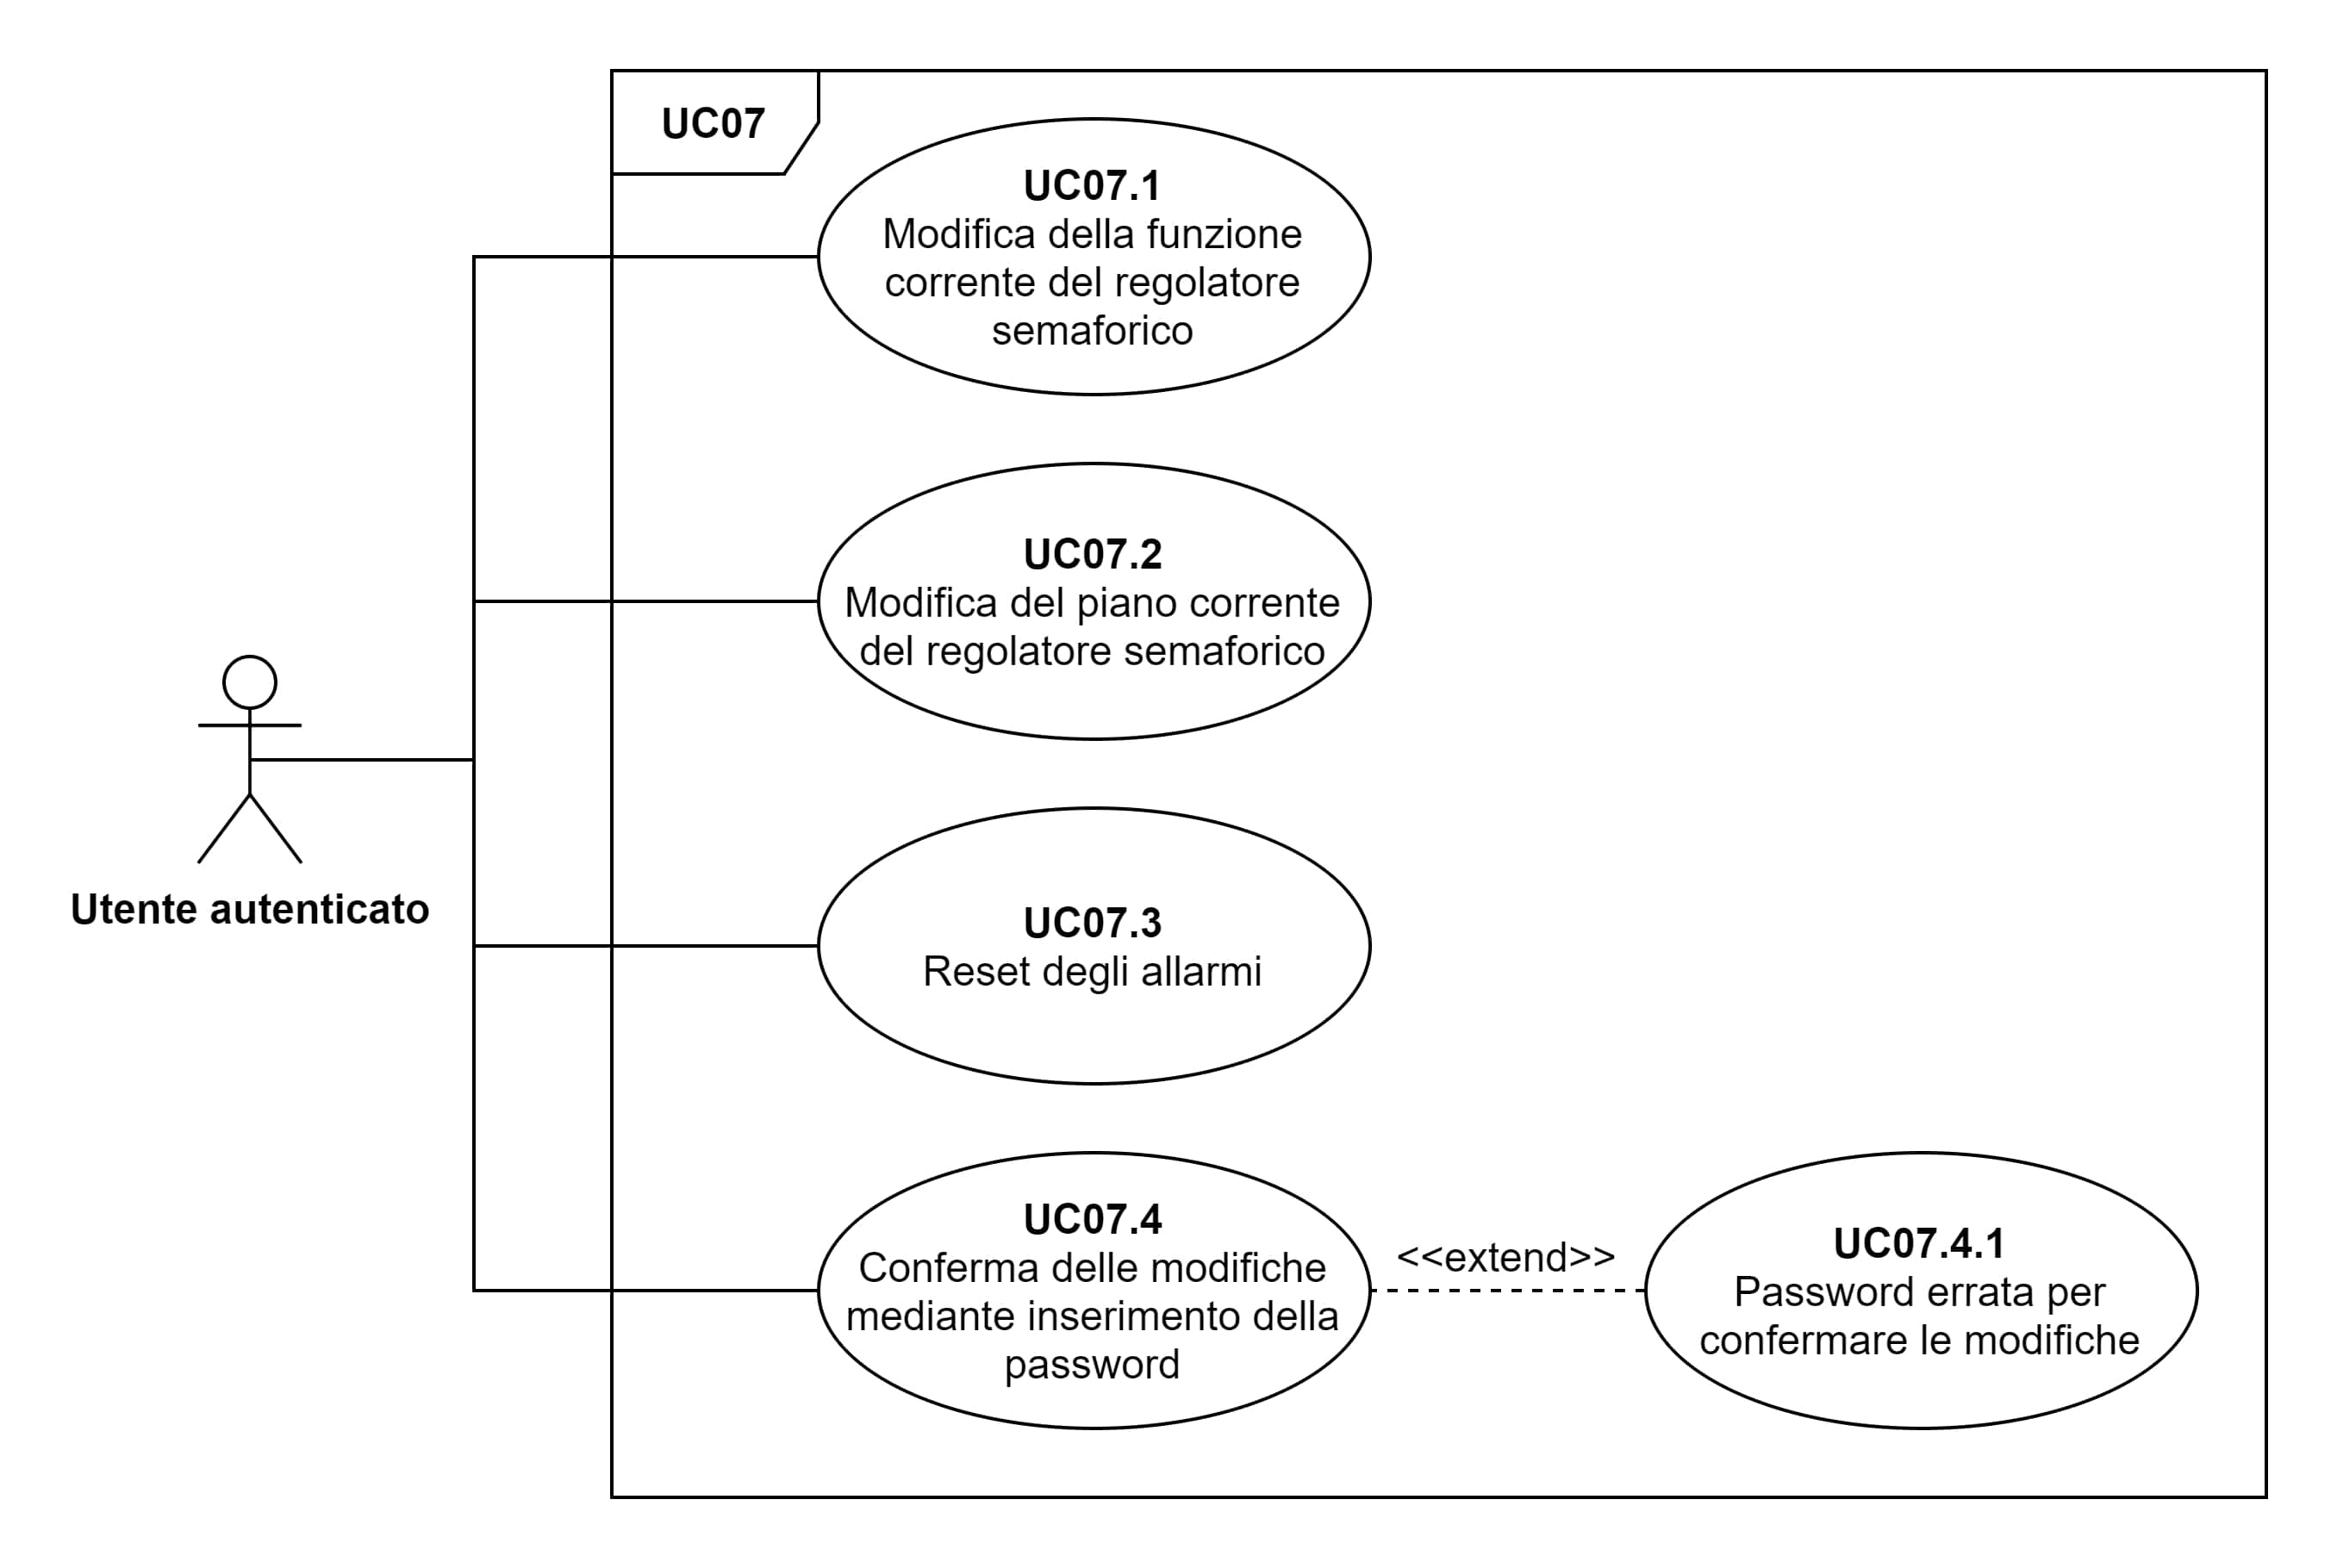
\includegraphics[width=1.0\columnwidth]{appendice-A/uc07} 
    \caption{SMacs - Sotto-casi d'uso di UC07 - Gestione del regolatore semaforico}
\end{figure}

\begin{usecase}{07.1}{Modifica della funzione corrente del regolatore semaforico}
\usecaseprimaryactors{Utente autenticato}
\usecasepre{L'utente ha a disposizione le funzionalità di gestione del regolatore semaforico.}
\usecasedesc{L'utente ha selezionato la funzionalità di modifica e ha aggiornato la funzione corrente del regolatore semaforico.}
\usecasepost{L'utente ha selezionato la funzionalità di modifica e ha aggiornato la funzione corrente del regolatore semaforico.}
\label{uc:UC07-1}
\end{usecase}

\begin{usecase}{07.2}{Modifica del piano corrente del regolatore semaforico}
\usecaseprimaryactors{Utente autenticato}
\usecasepre{L'utente ha a disposizione le funzionalità di gestione del regolatore semaforico.}
\usecasedesc{L'utente ha selezionato la funzionalità di modifica e ha aggiornato il piano corrente del regolatore semaforico.}
\usecasepost{L'utente ha selezionato la funzionalità di modifica e ha aggiornato il piano corrente del regolatore semaforico.}
\label{uc:UC07-2}
\end{usecase}

\begin{usecase}{07.3}{Reset degli allarmi}
\usecaseprimaryactors{Utente autenticato}
\usecasepre{L'utente ha a disposizione le funzionalità di gestione del regolatore semaforico.}
\usecasedesc{L'utente ha selezionato la funzionalità di reset e ha resettato gli allarmi relativi al regolatore semaforico attualmente registrati per il dispositivo.}
\usecasepost{L'utente ha selezionato la funzionalità di reset e ha resettato gli allarmi relativi al regolatore semaforico attualmente registrati per il dispositivo.}
\label{uc:UC07-3}
\end{usecase}

\begin{usecase}{07.4}{Conferma delle modifiche mediante inserimento della password}
\usecaseprimaryactors{Utente autenticato}
\usecasepre{L'utente ha modificato un'impostazione del regolatore semaforico.}
\usecasedesc{L'utente ha modificato un dato di funzionamento del regolatore semaforico e per confermarlo deve inserire la propria password.}
\usecasepost{L'utente ha modificato un dato di funzionamento del regolatore semaforico e per confermarlo ha inserito la propria password.}
\usecaseext{UC07.4.1}
\label{uc:UC07-4}
\end{usecase}

\begin{usecase}{07.4.1}{Password errata per confermare le modifiche}
\usecaseprimaryactors{Utente autenticato}
\usecasepre{L'utente ha inserito la propria password per confermare le modifiche.}
\usecasedesc{L'utente ha inserito una password errata, la modifica non viene confermata e viene avvisato con un messaggio di errore.}
\usecasepost{L'utente ha inserito una password errata, la modifica non viene confermata e viene avvisato con un messaggio di errore.}
\label{uc:UC07-4-1}
\end{usecase}

\begin{usecase}{08}{Lista degli eventi del regolatore semaforico}
\usecaseprimaryactors{Utente autenticato}
\usecasepre{L'utente sta visionando il dettaglio del regolatore semaforico selezionato dalla lista.}
\usecasedesc{Viene visualizzata la lista degli eventi relativi al regolatore semaforico selezionato per la data corrente.}
\usecasepost{Viene visualizzata la lista degli eventi relativi al regolatore semaforico selezionato per la data corrente.}
\label{uc:UC08}
\end{usecase}

\begin{figure}[!h] 
    \centering 
    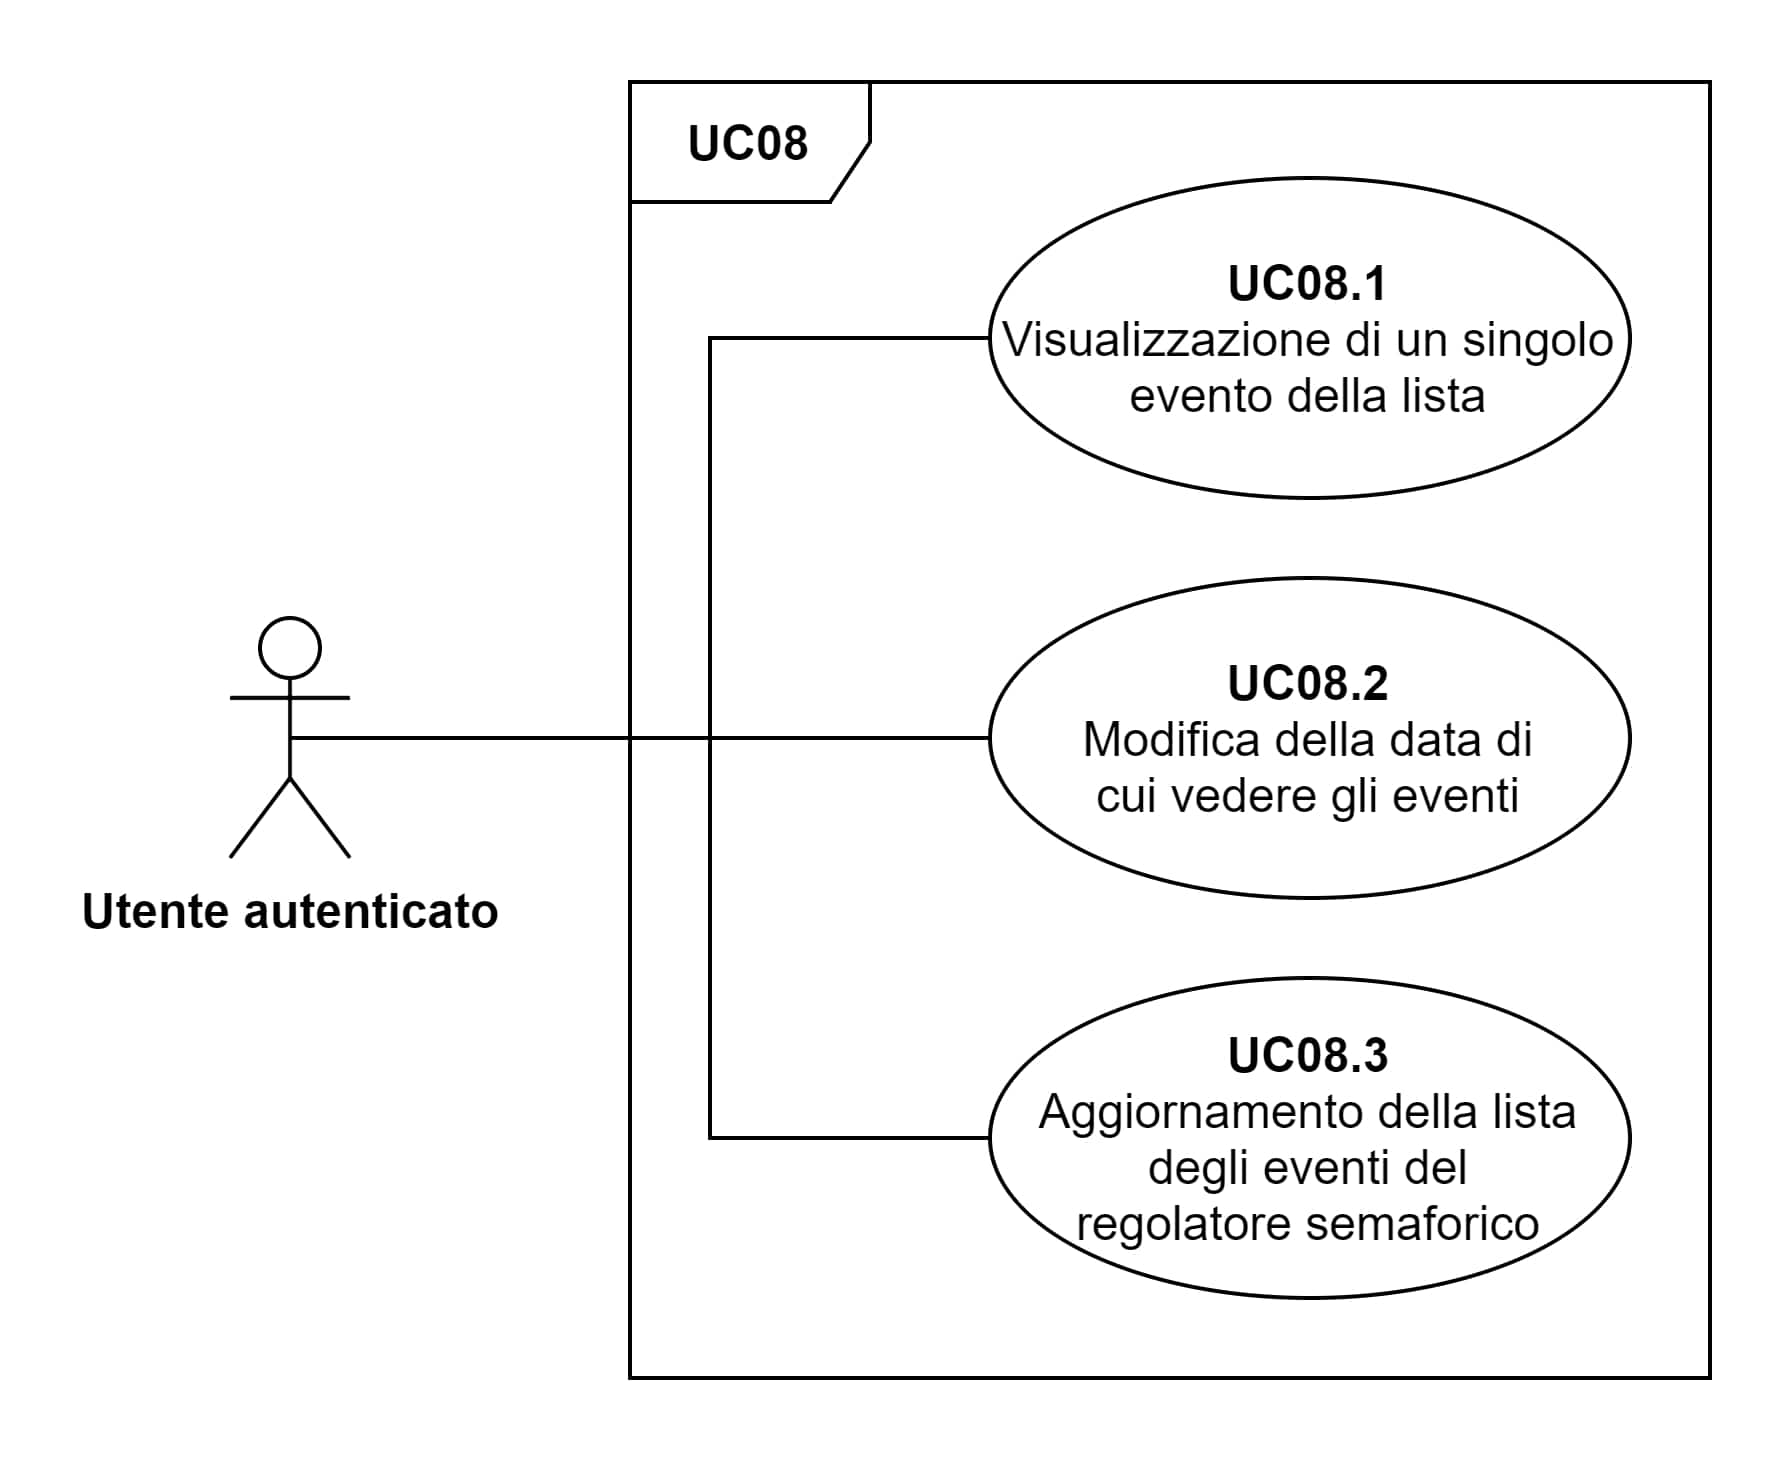
\includegraphics[width=1.0\columnwidth]{appendice-A/uc08} 
    \caption{SMacs - Sotto-casi d'uso di UC08 - Lista degli eventi del regolatore semaforico}
\end{figure}

\begin{usecase}{08.1}{Visualizzazione di un singolo evento della lista}
\usecaseprimaryactors{Utente autenticato}
\usecasepre{L'utente sta visionando la lista degli eventi del regolatore semaforico.}
\usecasedesc{Viene visualizzato un singolo evento relativo al regolatore semaforico della lista, mostrando un icona che rappresenta la gravità dell'evento e un breve messaggio descrittivo.}
\usecasepost{Viene visualizzato un singolo evento relativo al regolatore semaforico della lista, mostrando un icona che rappresenta la gravità dell'evento e un breve messaggio descrittivo.}
\label{uc:UC08-1}
\end{usecase}

\begin{usecase}{08.2}{Modifica della data di cui vedere gli eventi}
\usecaseprimaryactors{Utente autenticato}
\usecasepre{L'utente sta visionando la lista degli eventi del regolatore semaforico.}
\usecasedesc{L'utente seleziona la funzionalità di aggiornamento e aggiorna la data di visualizzazione degli eventi del regolatore semaforico.}
\usecasepost{L'utente seleziona la funzionalità di aggiornamento e aggiorna la data di visualizzazione degli eventi del regolatore semaforico.}
\label{uc:UC08-2}
\end{usecase}

\begin{usecase}{08.3}{Aggiornamento della lista degli eventi del regolatore semaforico}
\usecaseprimaryactors{Utente autenticato}
\usecasepre{L'utente sta visionando la lista degli eventi del regolatore semaforico.}
\usecasedesc{L'utente seleziona la funzionalità di aggiornamento e viene aggiornata la lista degli eventi del regolatore semaforico.}
\usecasepost{L'utente seleziona la funzionalità di aggiornamento e viene aggiornata la lista degli eventi del regolatore semaforico.}
\label{uc:UC08-3}
\end{usecase}

\begin{usecase}{09}{Visualizzazione del foglio di informazioni del dispositivo}
\usecaseprimaryactors{Utente autenticato}
\usecasepre{L'utente sta visionando il dettaglio del regolatore semaforico selezionato dalla lista.}
\usecasedesc{L'utente ha selezionato la funzionalità di visualizzazione del documento con le informazioni sul dispositivo che viene quindi mostrato.}
\usecasepost{L'utente ha selezionato la funzionalità di visualizzazione del documento con le informazioni sul dispositivo che viene quindi mostrato.}
\label{uc:UC09}
\end{usecase}

\begin{usecase}{10}{Visualizzazione posizione geografica del regolatore semaforico}
\usecaseprimaryactors{Utente autenticato}
\usecasesecondaryactors{Mappe del dispositivo}
\usecasepre{L'utente sta visionando il dettaglio del regolatore semaforico selezionato dalla lista.}
\usecasedesc{L'utente ha selezionato la funzionalità di visualizzazione della posizione geografica del regolatore semaforico e viene quindi reindirizzato all'applicazione di default delle mappe del dispositivo (smartphone/tablet) che visualizzerà quanto richiesto.}
\usecasepost{L'utente ha selezionato la funzionalità di visualizzazione della posizione geografica del regolatore semaforico e viene quindi reindirizzato all'applicazione di default delle mappe del dispositivo (smartphone/tablet) che visualizzerà quanto richiesto.}
\label{uc:UC10}
\end{usecase}

\begin{usecase}{11}{Visualizzazione di un testo riassuntivo sullo stato dei dispositivi}
\usecaseprimaryactors{Utente autenticato}
\usecasepre{L'utente ha ricevuto una notifica: quindi ha avviato l'applicazione oppure la stava già utilizzando (in qualsiasi modo).}
\usecasedesc{L'utente ha selezionato la funzionalità di visualizzazione di un testo riassuntivo della situazione attuale dello stato dei dispositivi collegati al suo account, mostrando anche i problemi (messaggi di diagnostica) presenti nuovi, presenti passati, risolti.}
\usecasepost{L'utente ha selezionato la funzionalità di visualizzazione di un testo riassuntivo della situazione attuale dello stato dei dispositivi collegati al suo account, mostrando anche i problemi (messaggi di diagnostica) presenti nuovi, presenti passati, risolti.}
\label{uc:UC11}
\end{usecase}

\begin{usecase}{12}{Gestione dell'intervallo di aggiornamento dati}
\usecaseprimaryactors{Utente autenticato}
\usecasepre{L'utente sta visionando la lista dei dispositivi collegati al proprio profilo.}
\usecasedesc{L'utente ha selezionato la funzionalità di gestione dell'intervallo di aggiornamento dati e ha aggiornato l'intervallo.}
\usecasepost{L'utente ha selezionato la funzionalità di gestione dell'intervallo di aggiornamento dati e ha aggiornato l'intervallo.}
\label{uc:UC12}
\end{usecase}

\begin{usecase}{13}{Informazioni sull'app}
\usecaseprimaryactors{Utente autenticato}
\usecasepre{L'utente sta visionando la lista dei dispositivi collegati al proprio profilo.}
\usecasedesc{L'utente ha selezionato la funzionalità di visualizzazione delle informazioni sull'applicazione e di cui viene visualizzata la versione e la data di rilascio, il server a cui si è connessi e l'username.}
\usecasepost{L'utente ha selezionato la funzionalità di visualizzazione delle informazioni sull'applicazione e di cui viene visualizzata la versione e la data di rilascio, il server a cui si è connessi e l'username.}
\label{uc:UC13}
\end{usecase}

\begin{usecase}{14}{Gestione della modalità di debug}
\usecaseprimaryactors{Utente autenticato}
\usecasepre{L'utente sta visionando la lista dei dispositivi collegati al proprio profilo.}
\usecasedesc{L'utente ha selezionato la funzionalità di gestione della modalità di debug e può attivarla o disattivarla, visionando dove i dati di debug verranno salvati.}
\usecasepost{L'utente ha selezionato la funzionalità di gestione della modalità di debug e può attivarla o disattivarla, visionando dove i dati di debug verranno salvati.}
\label{uc:UC14}
\end{usecase}

\begin{usecase}{15}{Logout dal sistema}
\usecaseprimaryactors{Utente autenticato}
\usecasepre{L'utente ha la possibilità di tornare un utente non autenticato.}
\usecasedesc{L'utente ha selezionato la funzionalità di logout e viene quindi disconnesso dal sistema.}
\usecasepost{L'utente ha selezionato la funzionalità di logout e viene quindi disconnesso dal sistema.}
\label{uc:UC15}
\end{usecase}

% \section{Tracciamento dei requisiti}

% Da un'attenta analisi dei requisiti e dei casi d'uso effettuata sul progetto è stata stilata la tabella che traccia i requisiti in rapporto ai casi d'uso.\\
% Sono stati individuati diversi tipi di requisiti e si è quindi fatto utilizzo di un codice identificativo per distinguerli.\\
% Il codice dei requisiti ha la forma $R\alpha{}x$ con $x$ numero naturale progressivo mentre $\alpha$ può essere:
% \begin{itemize}
%     \item F, che indica un requisito funzionale e obbligatorio, ovvero che implementa una funzionalità obbligatoria per il corretto funzionamento e completamento del prodotto;
%     \item D, che indica nuovamente un requisito funzionale ma desiderabile, ovvero che implementa una funzionalità che offre valore aggiunto ma che senza il prodotto può comunque portare a termine gli obiettivi per cui è stato creato;
%     \item Z, che indica ancora una volta un requisito funzionale però opzionale, ovvero che offre valore aggiunto ma che è subordinato dalla realizzazione degli altri requisiti, ed è quindi di inferiore importanza;
%     \item Q, che indica un requisito qualitativo, ovvero che garantisce un corretto funzionamento del prodotto secondo le attese dell'utente e degli stakeholder;
%     \item V, che indica un requisito vincolante per la buona riuscita del progetto e del prodotto, senza il cui completamento il prodotto non può ritenersi concluso.
% \end{itemize}
% Nelle tabelle \ref{tab:requisiti-funzionali}, \ref{tab:requisiti-qualitativi} e \ref{tab:requisiti-vincolo} sono riassunti i requisiti e il loro tracciamento con i casi d'uso delineati in fase di analisi.

% \newpage

% \begin{table}%
% \caption{Tabella del tracciamento dei requisiti funzionali}
% \label{tab:requisiti-funzionali}
% \begin{tabularx}{\textwidth}{lXl}
% \hline\hline
% \textbf{Requisito} & \textbf{Descrizione} & \textbf{Use Case}\\
% \hline
% RF01 & Viene visualizzata la schermata iniziale dell'applicazione quando l'utente non autenticato accede all'applicazione. & UC01 \\
% RF02 & Quando l'utente non autenticato si trova nella schermata iniziale dell'applicazione viene visualizzato il link per accedere al sito web dell'azienda. & UC01.1 \\
% RF03 & Quando l'utente non autenticato si trova nella schermata iniziale dell'applicazione viene visualizzato il modulo per contattare il servizio clienti. & UC01.2 \\
% RF04 & Quando l'utente non autenticato si trova nella schermata iniziale dell'applicazione viene visualizzato il link per accedere al sito web dell'azienda di cui è partner. & UC01.3 \\
% RF05 & Quando l'utente non autenticato si trova nella schermata iniziale dell'applicazione viene visualizzato la funzionalità di accesso alla schermata di autenticazione. & UC01.4 \\
% RF06 & L'utente non autenticato può autenticarsi presso il sistema. & UC02 \\
% RF07 & L'utente non autenticato può inserire il nome del server a cui connettersi. & UC02.1 \\
% RF08 & L'utente non autenticato può inserire il proprio nome utente per connettersi al sistema. & UC02.2 \\
% RF09 & L'utente non autenticato può inserire la propria password per connettersi al sistema. & UC02.3 \\
% RF10 & Se l'utente non autenticato si è dimenticato la propria password può accedere alla pagina web per contattare il servizio clienti. & UC02.4 \\
% RF11 & Se l'utente non autenticato ha inserito un server che non è valido viene visualizzato un messaggio di errore. & UC02.5 \\
% RF12 & Se l'utente non autenticato ha inserito delle credenziali che non sono valide viene visualizzato un messaggio di errore. & UC02.6 \\
% RF13 & L'utente autenticato può visionare la lista dei dispositivi di cui ha il permesso di gestione. & UC03 \\
% RF14 & L'utente autenticato può visionare un elemento della lista dei dispositivi comprensivo di un dettaglio compatto. & UC03.1 \\
% RF15 & L'utente autenticato è notificato quando la lista dei dispositivi di cui ha il permesso di gestione è vuota. & UC03.2 \\
% RF16 & L'utente autenticato può visionare la lista dei dispositivi di cui ha il permesso di gestione in ordine alfabetico. & UC03.3 \\
% RF17 & L'utente autenticato può visionare la lista dei soli dispositivi di cui ha il permesso di gestione che hanno segnalazioni (di malfunzionamento). & UC03.4 \\
% RF18 & L'utente autenticato può visionare la lista dei dispositivi entro il raggio di 1 Km dalla propria posizione di cui ha il permesso di gestione. & UC03.5 \\
% RF19 & L'utente autenticato può visionare la lista dei dispositivi filtrati in base a una ricerca testuale di cui ha il permesso di gestione. & UC03.6 \\
% RF20 & L'utente autenticato può aggiornare la lista dei dispositivi di cui ha il permesso di gestione ottenendone una nuova copia dal sistema. & UC03.7 \\
% RF21 & L'utente autenticato può ottenere informazioni dettagliate sullo stato di un regolatore semaforico. & UC04 \\
% RF22 & L'utente autenticato può ottenere informazioni sulla massima gravità fra i messaggi di diagnostica attivi nel dispositivo. & UC04.1 \\
% RF23 & L'utente autenticato può ottenere informazioni sullo stato del regolatore semaforico (funzione, livello). & UC04.2 \\
% RF24 & L'utente autenticato può ottenere informazioni sullo stato dei gruppi semaforici del regolatore semaforico. & UC04.3 \\
% RF25 & L'utente autenticato può ottenere informazioni sullo stato degli input presenti nel regolatore semaforico. & UC04.4 \\
% RF26 & L'utente autenticato può ottenere la data in cui è avvenuto l'ultimo aggiornamento dei dati del regolatore semaforico. & UC04.5 \\
% RF27 & L'utente autenticato può ottenere i messaggi di diagnostica presenti nel regolatore semaforico. & UC04.6 \\
% RF28 & L'utente autenticato può aggiornare lo stato del regolatore semaforico. & UC04.7 \\
% RF29 & L'utente autenticato può visionare il sinottico del regolatore semaforico. & UC05 \\
% RF30 & L'utente autenticato può gestire il dettaglio tecnico sul regolatore semaforico. & UC06 \\
% RF31 & L'utente autenticato può ottenere delle informazioni hardware e software delle componenti del regolatore semaforico. & UC06.1 \\
% RF32 & L'utente autenticato può ottenere informazioni sulla modalità di connessione attiva nel dispositivo. & UC06.2 \\
% RF33 & L'utente autenticato può ottenere informazioni sulle impostazioni DDNS del dispositivo. & UC06.3 \\
% RF34 & L'utente autenticato può aggiornare il dettaglio tecnico del regolatore semaforico. & UC06.4 \\
% RF35 & L'utente autenticato può inserire delle note sul dettaglio tecnico del regolatore semaforico. & UC06.5 \\
% RF36 & L'utente autenticato può gestire il regolatore semaforico. & UC07 \\
% RF37 & L'utente autenticato può modificare la funzione corrente del regolatore semaforico. & UC07.1 \\
% RF38 & L'utente autenticato può modificare il piano corrente del regolatore semaforico. & UC07.2 \\
% RF39 & L'utente autenticato può resettare gli allarmi del regolatore semaforico. & UC07.3 \\
% RF40 & L'utente autenticato può inserire la propria password per confermare le modifiche ai dati del regolatore semaforico. & UC07.4 \\
% RF41 & Se l'utente autenticato ha inserito la password e non corrisponde alla propria viene visualizzato un messaggio di errore. & UC07.4.1 \\
% RF42 & L'utente autenticato può visionare la lista degli eventi del regolatore semaforico. & UC08 \\
% RF43 & L'utente autenticato può visionare un singolo evento della lista. & UC08.1 \\
% RF44 & L'utente autenticato può modificare la data di cui vedere gli eventi del regolatore semaforico. & UC08.2 \\
% RF45 & L'utente autenticato può aggiornare la lista degli eventi del regolatore semaforico. & UC08.3 \\
% RF46 & L'utente autenticato può visionare il foglio contenente informazioni sul dispositivo. & UC09 \\
% RF47 & L'utente autenticato può visionare la posizione geografica del regolatore semaforico. & UC10 \\
% RF48 & L'utente autenticato può visionare un testo riassuntivo sullo stato dei dispositivi previa ricezione di una notifica. & UC11 \\
% RF49 & L'utente autenticato può gestire l'intervallo di aggiornamento dati. & UC12 \\
% RF50 & L'utente autenticato può visionare le informazioni sull'app. & UC13 \\
% RF51 & L'utente autenticato può gestire la modalità di debug. & UC14 \\
% RF52 & L'utente autenticato può effettuare il logout dal sistema. & UC15 \\
% \hline
% \end{tabularx}
% \end{table}%

% \begin{table}%
% \caption{Tabella del tracciamento dei requisiti qualitativi}
% \label{tab:requisiti-qualitativi}
% \begin{tabularx}{\textwidth}{lXl}
% \hline\hline
% \textbf{Requisito} & \textbf{Descrizione} & \textbf{Use Case}\\
% \hline
% RQD-1    & Le prestazioni del simulatore hardware deve garantire la giusta esecuzione dei test e non la generazione di falsi negativi & - \\
% \hline
% \end{tabularx}
% \end{table}%

% \begin{table}%
% \caption{Tabella del tracciamento dei requisiti di vincolo}
% \label{tab:requisiti-vincolo}
% \begin{tabularx}{\textwidth}{lXl}
% \hline\hline
% \textbf{Requisito} & \textbf{Descrizione} & \textbf{Use Case}\\
% \hline
% RVO-1    & La libreria per l'esecuzione dei test automatici deve essere riutilizzabile & - \\
% \hline
% \end{tabularx}
% \end{table}%